\documentclass[11pt,twocolumn]{article}
\usepackage{graphicx}
\usepackage[left=1.80cm, right=1.80cm, top=2.00cm, bottom=2.00cm]{geometry}
\usepackage{amsmath,bm}
\usepackage[colorlinks]{hyperref}
\usepackage[backend=biber, bibencoding=utf8]{biblatex}
\usepackage{eurosym}
\usepackage[dvipsnames]{xcolor}
\usepackage{subcaption}
\usepackage{booktabs} % for table (toprule, bottomrule)
\usepackage{enumitem} % for alphabetical enumeration 
\usepackage{accents}
\usepackage[capitalise]{cleveref}



\addbibresource{main.bib}
\graphicspath{{../figures/}{../figures/example/}}

\crefname{relation}{Rel.}{Rels.}
\creflabelformat{relation}{(#2#1#3)}
\crefname{constraint}{Constr.}{Constrs.}
\creflabelformat{constraint}{(#2#1#3)}
\crefname{subequations}{Eqs.}{Eqs.}
\creflabelformat{subequations}{(#2#1#3)}

\setlength\parindent{8pt}

% style operators
\newcommand{\ie}{\textit{i.e.} }
\newcommand{\eg}{\textit{e.g.} }
\newcommand{\ubar}[1]{\underaccent{\bar}{#1}}
\newcommand{\note}[1]{\textcolor{Orange}{#1}}
\newcommand{\vpad}{\vspace{1mm}}
\newcommand{\hpad}{\hspace{15pt}}
\newcommand{\resultsin}[1]{\hspace{6pt} \bot  \hspace{6pt} #1}
\newcommand{\Forall}[1]{\hspace{10pt} \forall \,\, #1 }
\newcommand{\pdv}[2]{\frac{\partial #1}{\partial #2}}



% general symbols
\newcommand{\state}{s_{i,t}}
\newcommand{\capacity}{S_{i}}
\newcommand{\costfactor}{\gamma_{i,t}}
\newcommand{\capacityupper}{\bar{S}}
\newcommand{\capacitylower}{\ubar{S}}
\newcommand{\muuppernom}{\bar{\mu}^\text{nom}_{i}}
\newcommand{\mulowernom}{\ubar{\mu}^\text{nom}_{i}}

%generation
\newcommand{\generation}{g_{s,t}}
\newcommand{\generationpotential}{\bar{g}_{s,t}}
\newcommand{\generationshare}[1][n]{\omega_{#1,s,t}}
\newcommand{\nodalgeneration}[1][n]{g_{#1,t}}
\newcommand{\capacitygeneration}{G_{s}}
\newcommand{\capacitygenerationupper}{\bar{G}_{s}}
\newcommand{\capacitygenerationlower}{\ubar{G}_{s}}
\newcommand{\operationalpricegeneration}{o_{s}}
\newcommand{\capitalpricegeneration}{c_{s}}
\newcommand{\mulowergeneration}{\ubar{\mu}_{s,t}}
\newcommand{\muuppergeneration}{\bar{\mu}_{s,t}}
\newcommand{\muuppergenerationnom}{\bar{\mu}^\text{nom}_{s}}
\newcommand{\mulowergenerationnom}{\ubar{\mu}^\text{nom}_{s}}


% flow
\newcommand{\flow}{f_{\ell,t}}
\newcommand{\capacityflow}{F_{\ell}}
\newcommand{\capacityflowUpper}{\bar{F}_{\ell}}
\newcommand{\capacityflowLower}{\ubar{F}_{\ell}}
\newcommand{\operationalpriceflow}{o_\ell}
\newcommand{\capitalpriceflow}{c_{\ell}}
\newcommand{\mulowerflow}{\ubar{\mu}_{\ell,t}}
\newcommand{\muupperflow}{\bar{\mu}_{\ell,t}}
\newcommand{\muupperflownom}{\bar{\mu}^\text{nom}_{\ell}}
\newcommand{\mulowerflownom}{\ubar{\mu}^\text{nom}_{\ell}}

% storage
\newcommand{\storage}{g_{r,t}}
\newcommand{\storagedispatch}{\storage^\text{dis}}
\newcommand{\storagecharge}{\storage^\text{sto}}
\newcommand{\storagesoc}{\storage^\text{ene}}
\newcommand{\storageprevioussoc}{g_{r,t-1}^\text{ene}}

\newcommand{\efficiency}{\eta_{r}}
\newcommand{\efficiencydispatch}{\efficiency^\text{dis}}
\newcommand{\efficiencycharge}{\efficiency^\text{sto}}
\newcommand{\efficiencysoc}{\efficiency^\text{ene}}

\newcommand{\operationalpricestorage}{o_r}
\newcommand{\capitalpricestorage}{c_r}
\newcommand{\capacitystorage}{G_r}
\newcommand{\capacitystorageupper}{\bar{G}_r}
\newcommand{\capacitystoragelower}{\ubar{G}_r}
\newcommand{\mulowerstorage}{\ubar{\mu}_{r,t}}
\newcommand{\muupperstorage}{\bar{\mu}_{r,t}}
\newcommand{\mulowerstoragedispatch}{\ubar{\mu}_{r,t}^\text{dis}}
\newcommand{\muupperstoragedispatch}{\bar{\mu}_{r,t}^\text{dis}}
\newcommand{\mulowerstoragecharge}{\ubar{\mu}_{r,t}^\text{sto}}
\newcommand{\muupperstoragecharge}{\bar{\mu}_{r,t}^\text{sto}}
\newcommand{\mulowerstoragesoc}{\ubar{\mu}_{r,t}^\text{ene}}
\newcommand{\muupperstoragesoc}{\bar{\mu}_{r,t}^\text{ene}}
\newcommand{\muupperstoragenom}{\bar{\mu}^\text{nom}_r}
\newcommand{\mulowerstoragenom}{\ubar{\mu}^\text{nom}_r}
\newcommand{\mustateofcharge}{\lambda^\text{ene}_{r,t}}
\newcommand{\munextstateofcharge}{\lambda^\text{ene}_{r,t+1}}


% other
\newcommand{\lagrangian}{\mathcal{L}}
\newcommand{\lmp}[1][n]{\lambda_{#1,t}}
\newcommand{\demand}[1][n]{d_{#1,t}}
\newcommand{\nodaldemand}[1][n]{d_{#1,t}}
\newcommand{\demandshare}[1][n]{\omega_{#1,a,t}}
\newcommand{\injection}{p_{n,t}}
\newcommand{\netconsumption}[1][n]{p^{-}_{#1,t}}
\newcommand{\netproduction}[1][n]{p^{+}_{#1,t}}
\newcommand{\selfconsumption}[1][n]{p^{\circ}_{#1,t}}
\newcommand{\totalnetconsumption}{p^{-}_{t}}
\newcommand{\totalnetproduction}{p^{+}_{t}}
\newcommand{\totalselfconsumption}{p^{\circ}_{t}}

% network
\newcommand{\incidence}[1][n]{K_{#1,\ell}}
\newcommand{\incidencegenerator}[1][n]{K_{#1,s}}
\newcommand{\incidencestorage}[1][n]{K_{#1,r}}
\newcommand{\incidenceasset}[1][n]{K_{#1,i}}
\newcommand{\ptdf}[1][n]{H_{\ell,#1}}
\newcommand{\cycle}{C_{\ell,c}}
\newcommand{\impedance}{x_\ell}
\newcommand{\cycleprice}{\lambda_{c,t}}



% Cost Terms
\newcommand{\emission}{e_{s}}
\newcommand{\emissionprice}{\mu_{\text{CO2}}}
\newcommand{\megawatthour}{MWh$_\text{el}$}
\newcommand{\totalcost}{\mathcal{TC}}
\newcommand{\cost}{\mathcal{C}}
\newcommand{\opex}{\mathcal{O}}
\newcommand{\opexgeneration}{\mathcal{O}^G}
\newcommand{\opexflow}{\mathcal{O}^F}
\newcommand{\opexstorage}{\mathcal{O}^E}
\newcommand{\capexgeneration}{\mathcal{C}^G}
\newcommand{\capexflow}{\mathcal{C}^F}
\newcommand{\capexstorage}{\mathcal{C}^E}
\newcommand{\emissioncost}{\mathcal{E}}
\newcommand{\remainingcost}{\mathcal{R}}
\newcommand{\scarcitycost}{\remainingcost^\text{scarcity}}
\newcommand{\subsidycost}{\remainingcost^\text{subsidy}}


% allocation quantities
\newcommand{\allocategeneration}[1][s, n]{A_{#1,t}}
\newcommand{\allocatestoragedispatch}[1][r, n]{A_{#1,t}}
\newcommand{\allocatepeer}[1][m \rightarrow n]{A_{#1,t}}
\newcommand{\allocateflow}[1][n]{A_{\ell,#1,t}}
\newcommand{\allocatetransaction}[1][s \rightarrow n]{A_{#1,\ell,t}}
\newcommand{\allocatestate}[1][i, n]{A_{#1,t}}

\newcommand{\allocatecost}[1][n \rightarrow i]{\cost_{#1, t}}
\newcommand{\allocatecapexgeneration}[1][n \rightarrow s]{\capexgeneration_{#1,t}}
\newcommand{\allocatecapexflow}[1][n \rightarrow \ell]{\capexflow_{#1,t}}
\newcommand{\allocatecapexstorage}[1][n \rightarrow r]{\capexstorage_{#1,t}}
\newcommand{\allocateopex}[1][n \rightarrow s]{\opex_{#1,t}}
\newcommand{\allocateemissioncost}[1][n \rightarrow s]{\emissioncost_{#1,t}}
\newcommand{\allocatescarcitycost}[1][n \rightarrow i]{\scarcitycost_{#1,t}}
\newcommand{\allocatesubsidycost}[1][n \rightarrow i]{\subsidycost_{#1,t}}



\begin{document}


\title{A dispatch-based approach to fully allocate costs in optimal power systems}
\author{F. Hofmann, Brown T.}

\maketitle

\begin{abstract}
% Maximizing the welfare of all market participants within a power system is a common approach in energy system modelling. It leads to perfectly scheduled operations of generators and ... 
\end{abstract}


\subsection*{Highlights}
\begin{itemize}
 \item The LMP always breaks down into contributions of different cost terms (OPEX, CAPEX, etc.) of the system.
 \item Breaking the LMP further down into contributions of components (generator, transmission line, etc.) requires assumptions on power flow assignments, where prominent methods as Average Participation or Flow Based Market Coupling can be applied.
 \item ...
 \item ...
\end{itemize}


% \section{Introduction}



\subsubsection*{Nomenclature}

\begin{table}[h]
    \centering
    \begin{tabular}{ll}
        $\lmp$ & Locational Market Price at bus $n$ and  \\ & time step $t$ in \euro/MW \vpad \\
        $\demand$ & Electric demand per bus $n$, demand type $a$, \\ & time step $t$ in MW  \vpad \\
        $\generation$ & Electric generation of generator $s$, \\ & time step $t$  in MW \vpad \\
        $\flow$ & Active power flow on line $\ell$, \\ & time step $t$ in MW   \vpad \\
        $\operationalpricegeneration$ & Operational price in \euro/MW \vpad \\
        $\capitalpricegeneration$ & Capital Price in \euro/MW \vpad \\
        $\capitalpriceflow$  & Capital Price in \euro/MW for transmission \\ & capacity on line $\ell$  \vpad \\
        $\capacitygeneration$ & Generation capacity in MW \vpad \\
        $\capacityflow$ & Transmission capacity in MW \vpad \\
        $\incidence$ & Incidence matrix \vpad 
    \end{tabular}
\end{table}

\section{Economic Context}

In long-term operation and investment planning models, the total costs $\totalcost$ of a power system is the sum of multiple cost terms. Typically, these include operational expenditures (OPEX) $\opexgeneration$ for generators, expenditures for emissions $\emissioncost$, capital expenditures (CAPEX) for generators $\capexgeneration$, CAPEX for the transmission system $\capexflow$ and possible other terms, \ie
\begin{align}
\totalcost &= \opexgeneration + \emissioncost +  \capexgeneration +  \capexflow + ...
\label{eq:total_cost}
\end{align}
In turn, each of these terms $\mathcal{C} = \{\opexgeneration, \emissioncost, \capexgeneration, \capexflow, ...\}$ consists of cost associated to the asset $i$ in the system, 
\begin{align}
    \cost = \sum_{i} \cost_{i}
    \label{eq:asset_cost}
\end{align} 
where an asset describes any component of the network, such as a generator, line, energy storage etc. %For example the total OPEX, $\opexgeneration = \sum_{s} \opexgeneration_{s}$, is the combined OPEX of all generators $s$.


In a cost-optimal setup with minimized $\totalcost$, the Locational Marginal Price (LMP) describes the price for an incremental increase of electricity demand $\demand$ at node $n$. It is given by the derivative of the total system cost $\totalcost$ with respect to the local demand $\demand$
\begin{align}
\lmp = \pdv{\,\totalcost}{\,\demand}
\label{eq:lmp}
\end{align}
% 
\begin{figure}[h]
\centering
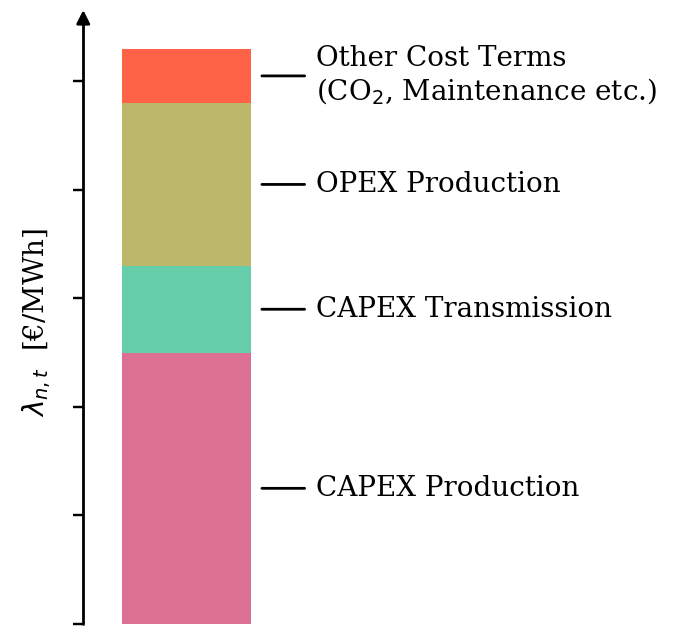
\includegraphics[width=.8\linewidth]{price_decomposition.png}
\caption{Schematic decomposition of the Locational Market Price $\lmp$. In power system model with optimal long-term operation and planning, the total system costs $\totalcost$ split into different cost terms, \ie OPEX and CAPEX for production and transmission and possibly other expenditures. }
\label{fig:price_decomposition}
\end{figure}
% 
This leads to a nodal pricing where over the span of optimized time steps $t$, the system costs are partially or totally payed back by the consumers 
\begin{align}
\totalcost - \remainingcost &=  \sum_{n,t} \lmp \, \demand
\label{eq:total_revenue}
\end{align}
depending on the costs $\remainingcost$ which are independent of the nodal demand  
\begin{align}
 \pdv{\remainingcost}{\demand} = 0
\end{align}
% 
Generally speaking, the cost term $\remainingcost$, not covered by the consumers, results from additional demands on the network design, such as capacity expansion limits or minimum share of one technology in the power mix. However, in most cases, where $\remainingcost \ll  \totalcost$, these play a minor role. 

From feeding \cref{eq:total_cost} into \cref{eq:lmp} it follows naturally that the LMP splits into contribution to the above mentioned cost terms. This relation, which we schematically show in \cref{fig:price_decomposition}, was already shown in extensive investigations of the LMP \cite{schweppe_spot_1988}. However the question of how the LMP can be decomposed into contributions of single cost terms $\cost_{i}$ associated with asset $i$ remains unanswered. This work aims at presenting and illustrating a an intuitive, peer-to-peer cost allocation including all network assets. 



\section{Dispatch-Based Cost Allocation}
\label{sec:theory}
\begin{subequations}\label[subequations]{eq:general_scheme}

Let $\cost_{i}$ denote a general cost term associated with asset $i$. Consider a long-term equilibrium in a power system with perfect competition, then, according to the zero-profit condition, each cost term $\cost_{i}$ can be considered as a cost-weighted sum of the operational state $s_{i,t}$ of asset $i$, \ie
\begin{align}
    \cost_{i} = \sum_t  \costfactor \, \state
    \label{eq:cost_decomposition}
\end{align}
where $\costfactor$ denotes a cost factor in \euro/MW. 
If $\cost_i$ describes the OPEX occasioned by asset $i$, the cost factor $\costfactor$ is simply given by the marginal operational price $o_i$. However, as we will show later, if it describes the CAPEX of asset $i$, $\costfactor$ is a composition of shadow prices $\mu_{i,t}$ given at the optimum. %As we will show later the composition of $\mu_{i,t}$ must be determined for each type of asset individually.


% where $\costfactor$ is either a fixed operational price or a composition of shadow prices
Following the implications of \cref{eq:lmp,eq:total_revenue},  we define the cost $\allocatecost$ that consumers at bus $n$ have pay to asset $i$ at time $t$, in order to compensate for $\cost_i$. This leads us to 
\begin{align}
    \allocatecost = \costfactor \,\pdv{\state}{\demand} \demand
    \label{eq:cost_allocation}
\end{align}
The derivative on the right hand side is defined through the sensitivity of the operational variable $\state$ at the optimum against changes in the demand. 
\begin{align}
    \allocatestate \rightarrow\pdv{\state}{\demand} \demand
    \label{eq:state_allocation}
\end{align}    
... may be interpreted as the amount of power that asset $i$ supplies demand $\demand$ with. It heavily relies on the derivative of the operational state with respect to the nodal demand $\partial \state / \partial \demand$. 
From the natural fact that the sum of all contributions must return the cost term, 
\begin{align}
    \cost_i = \sum_{n,t} \allocatecost
    \label{eq:cost_payback}
\end{align}
it follows that $\allocatestate$ must fulfill
\begin{align}
    \state = \sum_n \allocatestate
    \label{eq:state_allocation_constraint}
\end{align}
The last equation states that all power produced or processed by asset $i$ must be totally consumed by the network demand $\demand$.  
Finally, the total contribution from node $n$ at time $t$ to the cost term $\cost$ amounts 
\begin{align}
    \cost_{n,t} = \sum_i \allocatecost
\end{align}
\end{subequations}

\begin{table*}[t]
    \begin{center}
        \begin{tabular}{l|c|c|c|c|c}
        & $i$ & $\cost$ & $\cost_i$  & $\costfactor$ & $\state$  \\
        \toprule 
        OPEX Production & $s$ & $\opexgeneration$ & $\sum_{t} \operationalpricegeneration \, \generation$   & $\operationalpricegeneration$ & $\generation$ \\  
        OPEX Transmission  & $\ell$ & $\opexflow$ & $\sum_{t} \operationalpriceflow \, |\flow|  $ & $\operationalpriceflow$ & $|\flow|$ \\  
        OPEX Storage & $r$  & $\opexstorage$ & $\sum_{t} \operationalpricestorage \, \storagedispatch$ &  $\operationalpricestorage$ & $\storage$ \\
        \midrule   
        CAPEX Production & $s$ & $\capexgeneration$ & $ \capitalpricegeneration \capacitygeneration$ & $\muuppergeneration$ & $\generation$ \\
        CAPEX Transmission & $\ell$ & $\capexflow$ & $ \capitalpriceflow \capacityflow$ & $\left(\muupperflow - \mulowerflow \right)$ & $\flow$ \\
        CAPEX Storage & $r$ & $\capexstorage$ & $ \capitalpricestorage \capacitystorage$ & $ \muupperstoragedispatch - \mulowerstoragedispatch  + (\efficiencydispatch )^{-1} \mustateofcharge $ & $\storage$ \\
        \midrule
        Emission Cost & $s$ & $\emissioncost$ & $ \emissionprice \, \emission \, \generation$ & $\emissionprice \,\emission$ & $\generation$ \\
        % \bottomrule   
    \end{tabular}
    \end{center}
    \caption{Mapping of different cost terms to the cost allocation scheme given in \cref{eq:general_scheme}. These include OPEX \& CAPEX for production, transmission and storage assets in the network, as well as a cost term for the total Green House Gas (GHG) emissions.}
    \label{tab:cost_allocation_map}
\end{table*}
    
Now, assume a network with generators $s$, transmission lines $\ell$ and storage units $r$. Each asset $i = \{s, \ell, r\}$ adds an term for OPEX and a term for CAPEX to the total system cost $\totalcost$.

\subsection{OPEX Allocation}

Let the operational price for an asset $i$ be given by $o_i$. Then, for example the OPEX occasioned by generator $s$ is given by 
\begin{align}
    \opexgeneration_s = \sum_t \operationalpricegeneration \, \generation 
    \label{eq:opexgeneration}
\end{align}
where $\generation$ denotes its power generation at time $t$. As \cref{eq:opexgeneration} matches the form of \cref{eq:cost_decomposition} which allows us to use the above presented scheme in \cref{eq:general_scheme}. As a result we obtain 
\begin{align}
    \allocateopex[n \rightarrow s] &= 
   \operationalpricegeneration \,  \allocategeneration
\label{eq:allocate_opexGeneration_detailed}
\end{align}
which is the contribution of $\demand$ to the OPEX at generator $s$.
The quantity  
\begin{align}
 \allocategeneration = \pdv{\generation}{\demand} \, \demand
 \label{eq:allocate_peer}
\end{align}
can be considered as the power that is produced by generator $s$ and consumed at node $n$ at time $t$. \\
In the same manner, we can follow the scheme allocate OPEX for flow $\flow$ and storage unit dispatch $\storagedispatch$. As we assume a bidirectional flow on line $\ell$, the OPEX is set proportional to the absolute value of the flow. The upper section in \cref{tab:cost_allocation_map} shows the mapping of variables to \cref{eq:general_scheme} in order to define the full OPEX allocation. \\

The scheme works for all other cost attached to the operational state of an asset $i$. Given for example a fix price for emissions $\emissionprice$ in \euro\, per tonne-CO$_2$ equivalents, the cost term for emission adds up to 
\begin{align}
 \emissioncost = \emissionprice \, \sum_s  \emission \, \generation
\end{align}
where $\emission$ denotes the emission factor in tonne-CO$_2$ per \megawatthour\, of generator $s$.
The allocated payment for consumers at bus $n$ at time $t$ assigned to generator $s$ is then given by 
\begin{align}
 \allocateemissioncost = \emissionprice \, \emission \, \allocategeneration
\end{align}


\subsection{CAPEX Allocation}
For the CAPEX allocation, it becomes crucial to look at the individual relations between operational state $\state$ and the capacity limit. For all assets, let the capital price for one unit capacity expansion be denoted by $c_i$.  All quantities for the CAPEX allocation, which we now discuss in detail, are summarized in the middle section of \cref{tab:cost_allocation_map}.  

\subsubsection{Generators}

The nominal capacity $\capacitygeneration$ constrains the generation $\generation$ in the form of 
\begin{align}
\generation - \generationpotential \capacitygeneration  &\le 0 \resultsin{\muuppergeneration} \Forall{s,t} 
\label[constraint]{eq:upper_generation_capacity_constraint}\\ 
- \generation &\le 0 \resultsin{\mulowergeneration} \Forall{s,t} 
\label[constraint]{eq:lower_generation_capacity_constraint}
\end{align}
where $\generationpotential \in \left[ 0,1\right]$ is the capacity factor for renewable generators. At a cost-optimum, these two constraints yield the shadow prices $\muuppergeneration$ and $\mulowergeneration$.  As shown in \cite{brown_decreasing_2020} and in detailed in \cref{sec:zero_profit_generation}, over the whole time span, the CAPEX for generator $s$ is payed back by the production $\generation$ times the shadow price $\muuppergeneration$, 
\begin{align}
 \capexgeneration_s = \capitalpricegeneration \capacitygeneration = \sum_t \muuppergeneration \,  \generation 
 \label{eq:no_profit_capex_generation}
\end{align}
This representation connects the CAPEX with the operational state of generator $s$, \ie matches the form in \cref{eq:cost_decomposition} allows for using the cost allocation scheme. The resulting the CAPEX allocation is given by
\begin{align}
 \allocatecapexgeneration = \muuppergeneration \, \allocategeneration
 \label{eq:allocate_capexGeneration_detailed}
\end{align}
How does this allocation behave? According to the polluter pays principle, it differentiates between consumers who are `responsible` for investments and those who are not. If $\muuppergeneration$ (in literature often denoted as the Quality of Supply) is bigger than zero, the upper Capacity \cref{eq:upper_generation_capacity_constraint} is binding. Thus it is these times steps which push investments in $\capacitygeneration$. If $\muuppergeneration = 0$, the generation $\generation$ is not bound and investments are not necessary. 
When summing over all CAPEX payments to generator $s$ in \cref{eq:allocate_capexGeneration_detailed} , we can use \cref{eq:state_allocation_constraint,eq:no_profit_capex_generation} to see that each generator retrieves exactly the cost that were spent to build the capacity $\capacitygeneration$.
 

\subsubsection{Transmission Lines}

The transmission capacity $\capacityflow$ limits the flow $\flow$ in both directions,
\begin{align}
\flow - \capacityflow &\le 0 \resultsin{\muupperflow} \Forall{\ell,t} 
\label[constraint]{eq:upper_flow_capacity_constraint} \\
- \flow - \capacityflow &\le 0 \resultsin{\mulowerflow} \Forall{\ell,t} 
\label[constraint]{eq:lower_flow_capacity_constraint}
\end{align}
which yield the shadow prices $\muupperflow$ and $\mulowerflow$. Again, we use the result of \cite{brown_decreasing_2020} (for details see \cref{sec:zero_profit_flow}) which derives that over the whole time span, the investment in line $\ell$ is payed back by the shadow prices times the flow 
\begin{align}
\capexflow_\ell = \capitalpriceflow \capacityflow = \sum_{t} \left( \muupperflow - \mulowerflow \right)  \flow 
\label{eq:no_profit_capex_flow}
\end{align}
From here, we follow the scheme in \cref{eq:general_scheme} which finally defines the CAPEX allocation as 
\begin{align}
    \allocatecapexflow &=  
   \left( \muupperflow - \mulowerflow\right) \, \allocateflow
   \label{eq:allocate_capexFlow_detailed}
\end{align}
The quantity 
\begin{align}
 \allocateflow =  \pdv{\flow}{\demand}\, \demand
\end{align}
can be interpreted as the flow that the demand at node $n$ and time $t$ causes on line $\ell$.
% According to \cref{eq:state_allocation_constraint} it has to fulfill 
% \begin{align}
%  \flow = \sum_{n} \allocateflow
% \label{eq:allocate_flow_constraint}
% \end{align}
The  shadow prices $\muupperflow$ and $\mulowerflow$ again can be seen as a measure for necessity of transmission investments at $\ell$ at time $t$. Hence, the definition of $\allocatecapexflow$ states that consumers, which retrieve power flowing on congested lines, yielding a bound \cref{eq:upper_flow_capacity_constraint} or \eqref{eq:lower_flow_capacity_constraint}, pay compensations for the resulting investments at $\ell$. Again the sum of all CAPEX payments to line $\ell$ equals the total CAPEX spent. This is seen when summing \cref{eq:allocate_capexFlow_detailed} over all buses and time steps and using \cref{eq:state_allocation_constraint,eq:no_profit_capex_flow}


\subsubsection{Storages}

% The complementary slackness of the above constraints,  
% \begin{align}
%     \capexstorage_r = \capitalpricestorage \, \capacitystorage = \sum_t \muupperstoragedispatch \, \storagedispatch + \muupperstoragecharge \, \storagecharge + \muupperstoragesoc \, \storagesoc
% \end{align}

In a simplified storage model, $\capacitystorage$ limits the storage dispatch $\storagedispatch$ and charging $\storagecharge$. Further it limits the maximal storage capacity $\storagesoc$ by a fix ratio $h_r$, denoting the maximum hours at full discharge. The storage $r$ dispatches power with efficiency $\efficiencydispatch$, charges power with efficiency $\efficiencycharge$ and preserves power from one time step $t$ to the next, $t+1$, with an efficiency of $\efficiencysoc$. In \cref{sec:zero_profit_storage_units} we formulate the mathematical details. As already shown in \cite{brown_decreasing_2020}, the total expenditures at $r$ are fully paid back by differences of the LMP at which the storage ``buys`` and ``sells`` power. Taking only the CAPEX into account the zero profit condition reduces to
\begin{align}
    \notag
    \capexstorage =& \capitalpricestorage \, \capacitystorage \\
    \notag
    =& \sum_t \left(\muupperstoragedispatch - \mulowerstoragedispatch  + (\efficiencydispatch )^{-1} \mustateofcharge \right) \storagedispatch \\
    &- \sum_t \lmp \incidencestorage  \storagecharge \Forall{r} 
    \label{eq:no_profit_capex_storage}
\end{align}
where $\muupperstoragedispatch$ and $\mulowerstoragedispatch$ are the shadow prices of the upper and lower dispatch capacity bound and $\mustateofcharge$ is the shadow price of the energy balance constraint. When applying the cost allocation scheme \cref{eq:general_scheme}, it stands to reason to assume that $\partial \storagecharge / \partial \demand \cdot \demand = 0$, implying that the when a storage charges power, it does not supply any demand. Rather it stands with the demand on the consumer side, retrieving power from producing assets. 
This leaves us with 
\begin{align}
     \allocatecapexstorage = \left(\muupperstoragedispatch - \mulowerstoragedispatch  + (\efficiencydispatch )^{-1} \mustateofcharge \right) \allocatestoragedispatch
\end{align}
and the power allocation 
\begin{align}
    \allocatestoragedispatch = \pdv{\storagedispatch}{\demand} \demand
\end{align}
The latter only allocates dispatched power of storage $r$. Note that this will break \cref{eq:cost_payback} as the payments to $r$ surpass the CAPEX by an amount $\remainingcost^E_r$. 
% \begin{align}
%     \capexstorage_r + \remainingcost^E_r = \sum_n \allocatecapexstorage
% \end{align} 
It is crucial to note that like this, storage units perform a redistribution of money, and therefore distort the cost allocation. So, certain share of what is allocated to the CAPEX of a storage is in another time step spent by the storage in order to buy power from other assets. This effect scales with the amount of installed capacity.

It is possible to incorporate this redistribution effect into the cost allocation, by replacing the demand $\demand$ with the power charge $\storagecharge$ in \cref{eq:general_scheme}. Then, the derived payments that a storage unit $r$ has to pay to asset $i$ is given by $\cost_{r \rightarrow i}$. The sum of those payments due to $r$ will the sum up to $\remainingcost^E_r$. 

% In a final step we can still allocate all cost to the demand $\demand$. However, this would require knowledge about when the power $\storagedispatch$ was initially charged: Given the amount of power $A_{r, t_{in} \rightarrow t_{out}}$ that is charged by storage $r$ at time step $t_{in}$ and discharged at $t_{out}$ ... 



\subsection{Design Constraints}

Power system modelling does rarely follow a pure Greenfield approach with unlimited capacity expansion. Rather, today's models are setting various constraints defining socio-political or  technical requirements. As mentioned before this will alter the equality of total cost and total revenue, \ie leads to $\remainingcost \ne 0$ in \cref{eq:total_revenue}. More precisely, each constraint $h_j$ (other then the nodal balance constraint) of the form 
\begin{align}
    h_j \left(\state, \capacity \right) - K < 0
\end{align}
where $K$ is any non-zero constant, will result in a cost term contributing to $\remainingcost$ and in some cases alter \cref{eq:cost_decomposition} to 
\begin{align}
    \cost_i - \remainingcost_i = \sum_t \costfactor \, \state
\end{align}
In the following we highlight two often used classes of constraints and show how to incorporate them into the cost allocation.  

\subsubsection{Capacity Expansion Limit}

In more realistic setups, generators, lines or other assets can only be built up to a certain limit. This might be due to land use restrictions or social acceptance problems. %In the following give a general solution how the cost allocation may handle this.  
However, when constraining the capacity $\capacity$  for a subset $I$ of assets to an upper limit $\capacityupper$, in the form of 
\begin{align}
    \capacity - \capacityupper \le 0 \resultsin{\muuppernom} \Forall{i \in I}
\label{eq:capacityexpansionmaximum},
\end{align}
the zero profit condition alters as soon as the constraint becomes binding. Then, the revenue of asset $i$ exceeds its total expenditures (OPEX + CAPEX). More precisely, the allocated CAPEX in \cref{tab:cost_allocation_map} will surpass the actual CAPEX of asset $i$ by the cost it has to pay for the scarcity, given by the absolute value of 
\begin{align}
    \scarcitycost_i = - \muuppernom \capacity \Forall{i \in I}
    \label{eq:scarcitycost}
\end{align}
% \begin{align}
%  \cost_i - \remainingcost_i =  \sum_t \costfactor \, \state \Forall{i}
%  \label{eq:capex_generation_duality_bf2}
% \end{align}

% In order to ensure that the allocated CAPEX sum up to the actual CAPEX at asset $i$, meaning that \cref{eq:cost_payback} holds, we adjust the CAPEX allocations to 
% \begin{align}
%     \allocatecost = \left(\dfrac{c_i}{c_i + \muuppernom}\right) \, \costfactor \, \allocatestate \Forall{i \in I}
% \end{align}
% with the cost factors $\costfactor$ for CAPEX given in \cref{tab:cost_allocation_map}. 
% The costs which consumers at $n$ have to pay for the scarcity impacting asset $i$ are given   
% \begin{align}
%     \allocatescarcitycost = \left(\dfrac{\muuppernom}{c_i + \muuppernom}\right) \, \costfactor \, \allocatestate \Forall{i \in I}
% \end{align}

The costs which consumers at $n$ have to pay for the scarcity impacting asset $i$ are given by 
\begin{align}
    \allocatescarcitycost = \dfrac{\muuppernom}{c_i + \muuppernom} \, \allocatecost^I \Forall{i \in I}
\end{align}
where $\allocatecost^I$ denotes the CAPEX allocation presented above. 

% have to be adjusted, as otherwise consumers would pay too much. As we show in ... updating the prices by a fix ratio 
% \begin{align}
%     \costfactor \rightarrow \dfrac{c_i}{c_i + \muuppernom}\, \costfactor
%     \label{eq:adjustment_lowernom}
% \end{align}
% will . Note that $\muuppernom$ is a positive number, so the adjustment cannot increase the paid price. 


\subsubsection{Brownfield Constraints}

In order to take already built infrastructure into account, the capacity $\capacity$ can be constrained to a minimum required capacity $\capacitylower$. Mathematically this translates to 
\begin{align}
    \capacitylower - \capacity  \le 0 \resultsin{\mulowernom} \hpad \forall{i \in I}
\label{eq:capacityexpansionminimum}
\end{align}
Again, such a setup alters the zero profit condition of asset $i$, as soon as the constraint becomes binding. 
In that case, asset $i$ does not collect enough revenue in order to match the CAPEX. The difference, given by 
\begin{align}
    \subsidycost_i = \mulowernom \capacity
    \Forall{i}
\end{align}
has to be subsidized by governments or communities. It is rather futile wanting to allocate these cost to consumers as assets may not gain any revenue for their operational state, \ie where $\cost^I = \subsidycost_i $. 


% Again, we can balance this effect out by updating the cost factor to 
% \begin{align}
%     \costfactor \rightarrow \costfactor +  \dfrac{\mulowernom \capacity}{\sum_t \state}
% \end{align}
% In contrast to \cref{eq:adjustment_lowernom} the price is not weighted by a factor but shifted for all time steps. This is required as 
% As $\mulowernom$ is a positive number, this will increase the price and therefore the revenue for asset $i$. 

% In order to take this effect into account for the cost allocation, we update the cost factors in \cref{tab:cost_allocation_map} to  

% \begin{align}
%     \costfactor \rightarrow \dfrac{c_i}{c_i + \muuppergenerationnom}\, \costfactor
% \end{align}
% This ensures that the allocated CAPEX sum up to the actual CAPEX at asset $i$ (and \cref{eq:cost_payback} holds).



\section{Assumptions on Power Allocations}
% \section{\texorpdfstring{Extended Solution Space of $\boldsymbol{\slackk[m]}$}{Solution Space of the Slack}}
\label{sec:localizing_allocations}

The presented cost allocation suits for any type of topology and network setup. But so far, the question of how $\allocatestate$ for generators $s$, lines $\ell$ and storages $r$ are defined was left open. We recap that all rely on derivatives of $\generation$, $\flow$ and $\storagedispatch$  with respect to the nodal demand $\demand$ (see \cref{eq:state_allocation_constraint}). \\

Let $\nodalgeneration[m]$ denote the nodal power generation which combines the power production of all producing assets, in this case generators $S$ and storages $R$, at node $n$ and time $t$. It is given by 
\begin{align}
    \nodalgeneration[m] = \sum_{i \in \{S, R\}} \incidenceasset[m] \, \state
\end{align}
with $\incidenceasset[m]$ being 1 if asset $i$ is attached to bus $m$ and zero otherwise. Further, let $\allocatepeer$ collect the power produced by assets at node $m$ and consumed at $n$, given by 
\begin{align}
    \allocatepeer = \sum_{i \in \{S,R\}} \incidenceasset[m] \, \allocatestate  
    % \nodalgeneration[m] = \sum_s \incidencegenerator[m] \, \generation + \sum_r \incidencestorage[m] \storagedispatch \Forall{n}
\end{align}
Now, let $\ptdf$ denote Power Transfer Distribution Factors (PTDF) giving the changes in the flow on line $\ell$ for one unit (typically one MW) of net power production at bus $n$. The linear power flow equation can be written as 
\begin{align}
 \flow  = \sum_m \ptdf[m] \left( \nodalgeneration[m] - \demand[m] \right)  
\end{align}
Note that for transport models or mixed AC-DC networks, $\ptdf$ can be artificially calculated using the formulation presented in \cite{hofmann_flow_2020-1}.
Taking the derivative with respect to the demand, 
\begin{align}
 \allocateflow = \pdv{\flow}{\demand} \demand = \sum_m \ptdf[m] \left( \allocatepeer  - \delta_{n,m} \demand \right) 
 \label{eq:allocate_peer_to_allocate_flow},
\end{align}
shows that $\allocateflow$ is fully determined through the peer-to-peer allocation $\allocatepeer$. In other words, we only need to know how much power produced at node $m$ is consumed at node $n$ in order to derive the allocated flow $\allocateflow$. Further we can breakdown $\allocatepeer$ to $\allocategeneration$ for generators and $\allocatestoragedispatch$ for storages proportionally to their contribution to the nodal generation $\nodalgeneration[m]$. Unfortunately, the solution for $\allocatepeer$ is non-unique and requires further assumptions. Established flow allocation schemes approach this problem from different directions. Principally two options exist \textit{what} is allocated 
% 
\begin{enumerate}
\item gross power injections \label{gross}
\item net power injections \label{net}
\end{enumerate}
% 
Further it is important \textit{what assumptions} define the allocation, \ie what method is used to define the pairs of sources and sinks. The three suitable approaches we present here are
% 
\begin{enumerate}[label=\alph*., ref=\alph*]
\item Equivalent Bilateral Exchanges (EBE) \cite{galiana_transmission_2003} which assumes
that every producer supplies every consumer proportional to its share in the total consumption. \label{ebe} 
\item Average Participation (AP) \cite{bialek_tracing_1996,achayuthakan_electricity_2010} which traces the flow from producer to consumer following the law of proportional sharing. \label{ap}
\item Flow Based Market Coupling (FBMC) which uses zonal PTDF for allocating power within predefined regions. The interregional exchange is only allocating net power deficit or excess of the regions. \label{fbmc}
\end{enumerate}
% 
We show the mathematical formulation for all combinations \ref{ebe}\ref{gross} - \ref{fbmc}\ref{net} in \cref{sec:gross_ebe,sec:net_ebe,sec:gross_ap,sec:net_ap}.
% 
Principally, type \ref{net} leads to less P2P trades then type \ref{gross} as power from a bus $m$ with $\nodalgeneration[m] \le \nodaldemand[m]$ is not assigned to other buses, only to $m$. 
Further, as literature has often pointed out, the EBE principal \ref{ebe} does not suit for large networks where remote buses would interconnect in the same way as buses in close vicinity \cite{gil_multiarea_2005}. The AP based type \ref{ap} tackles this problem by restricting P2P trades to those which are traceable when applying the proportional sharing principal. Therefore $\allocategeneration$ denotes that part of power produced by bus $m$ which, when only following in the direction of $\flow$, ends up at bus $n$. Type \ref{fbmc} further allows to control the regions or market zones which are netted out in a first step. If in a region $R$ the generation undercuts the demand, $\sum_{n \in R} \nodalgeneration \le \sum_{n \in R} \demand$, none of the inner-regional generation is assigned to other regions. However, it relies on further assumptions such as the Generation Shift Keys determining the production which are deployed for the inter-regional exchange. 
From this point of view, we set the main focus of this research to the AP based scheme, as locality and little de-pendency on external decisions are strong arguments for a transparent cost allocation. However, we will use the EBE based cost allocation for the following example, in order to depict the functionality of the cost allocation and the fundamental difference between the allocation of gross and net power. 

\subsection{Numerical Example}
\label{sec:numerical_example}

\begin{figure*}[t]
    \centering
    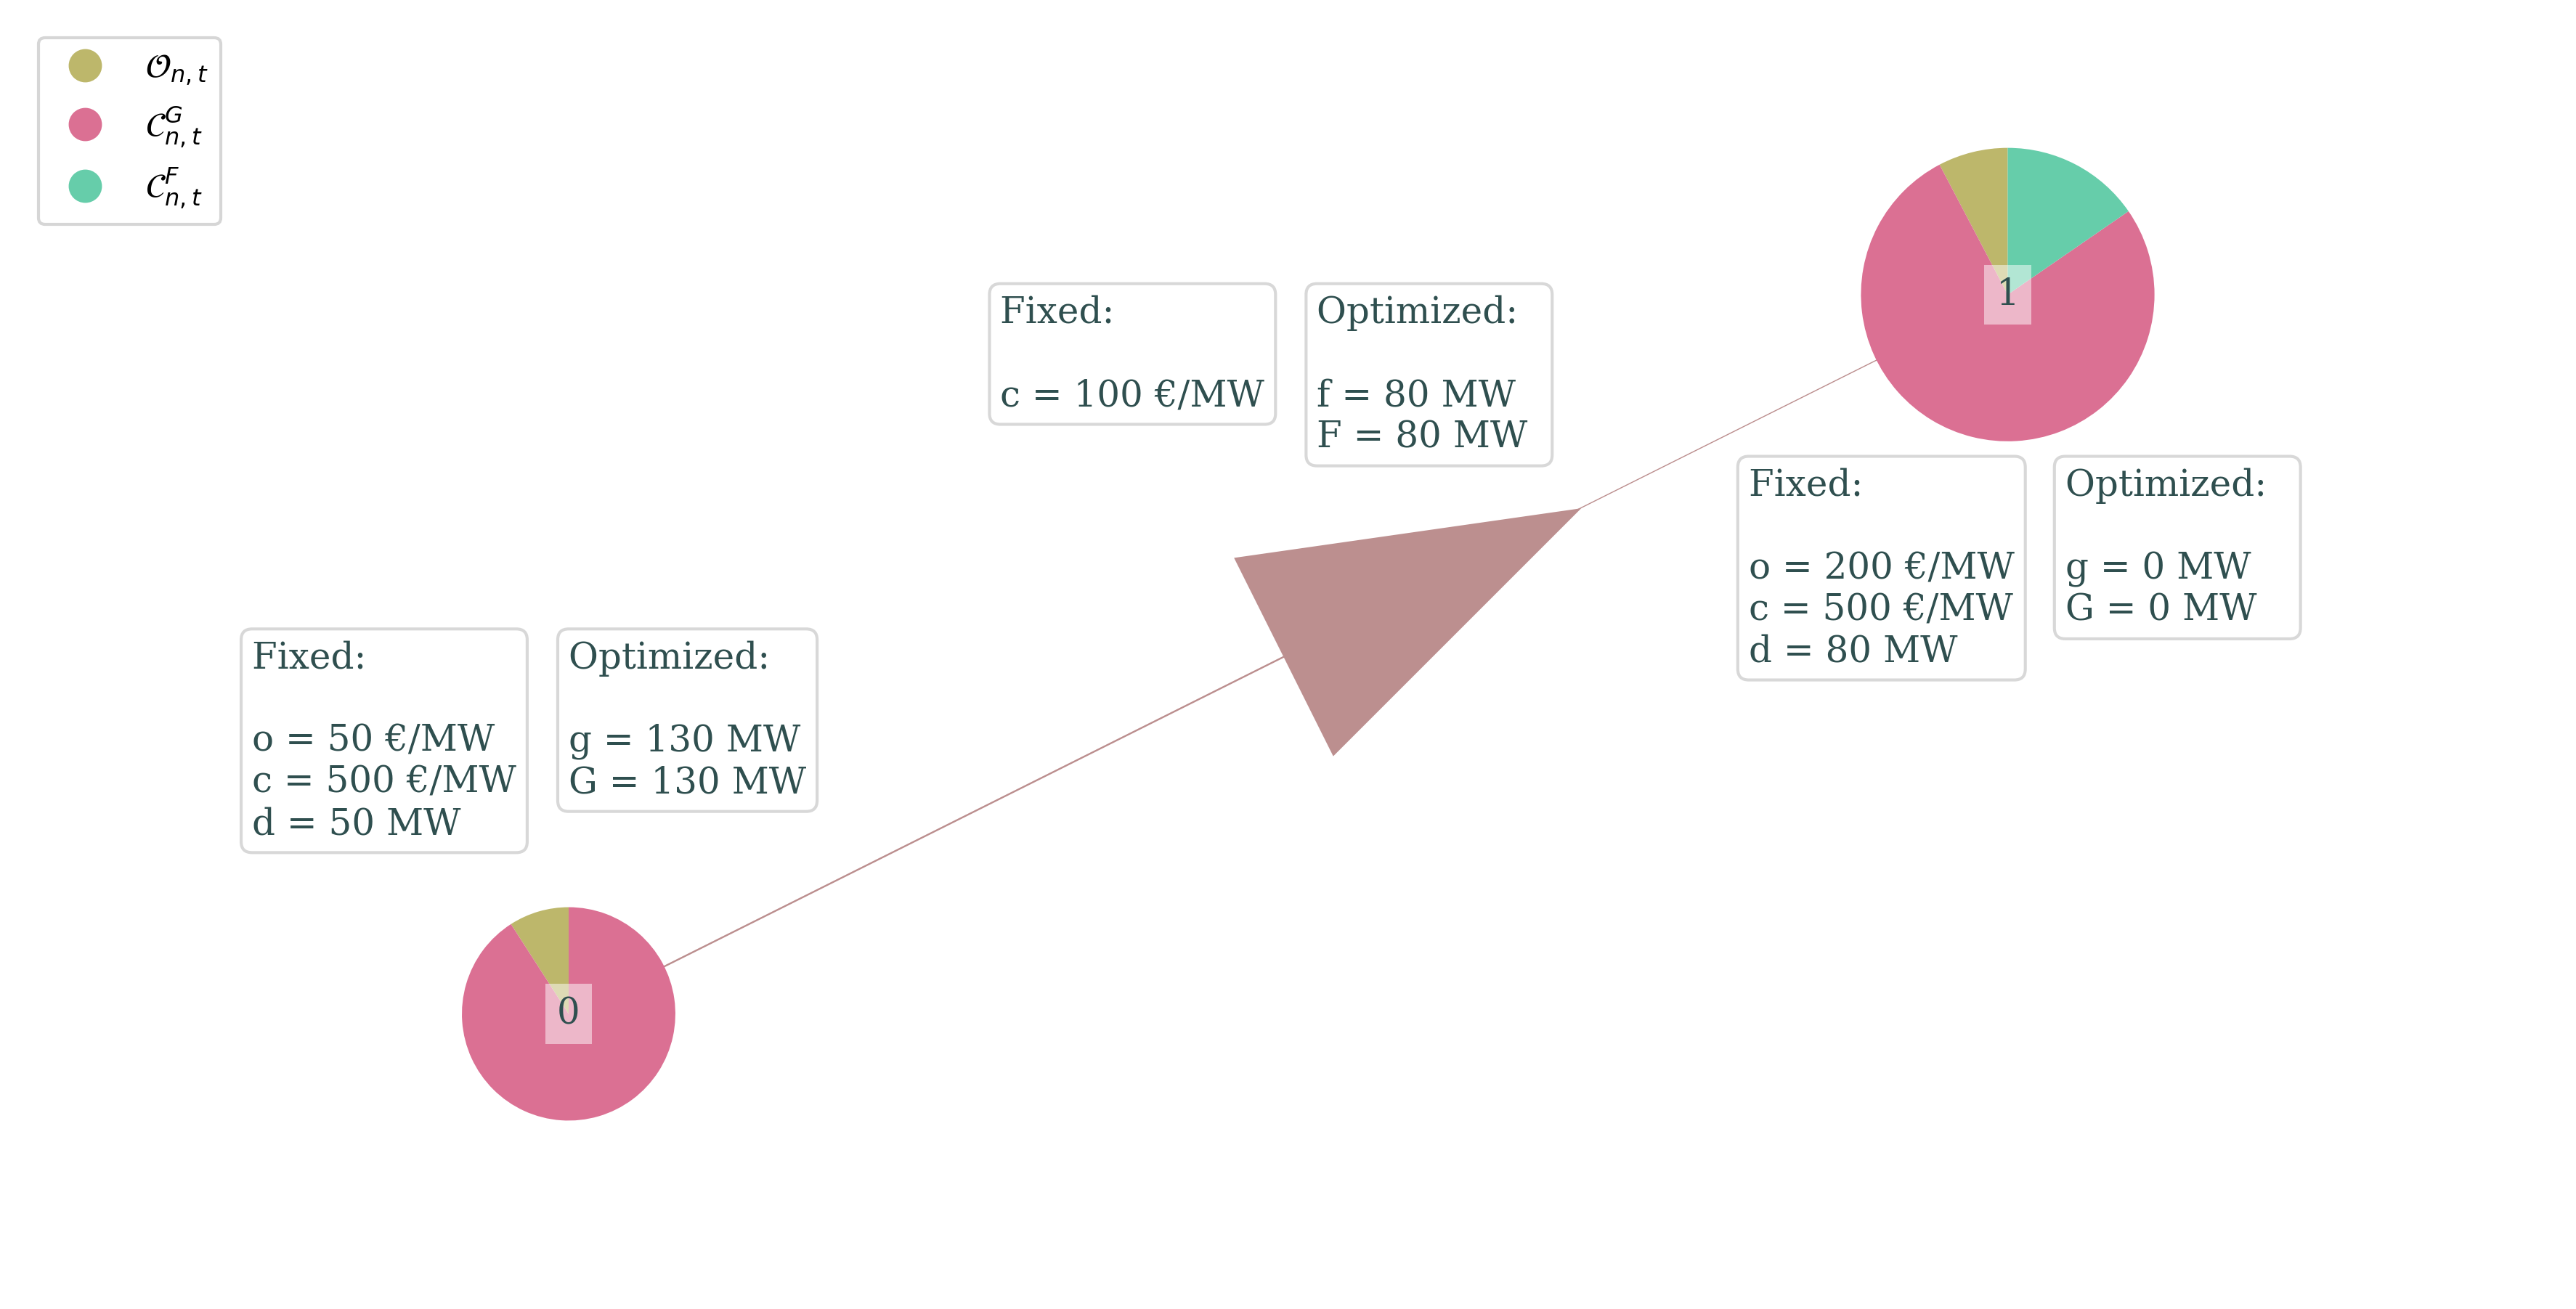
\includegraphics[width=\linewidth]{example_network.png}
    \caption{Illustrative example of a 2-bus network with one optimized time step. Fixed prices and constraining values are given in the left box for each bus and the transmission line. Optimized values are given in the right boxes. Bus~1 has a cheaper operational price $o$, capital prices are the same for both. As both generator capacities are constraint to 100~MW, the optimization also deploys the generator at bus~2. The resulting electricity prices $\lambda$ are then a composition of all prices for operation and capital investments.}
    \label{fig:example_network}
    \end{figure*}
    % 
% 
% 
Consider a two bus system, as shown in \cref{fig:example_network}, with one transmission line and one generator per bus. Whereas generator~1 (at bus~1) has an operational price of 50 \euro/\megawatthour, generator~2 (at bus~2) has a higher operational price of 200~\euro/\megawatthour. For both the CAPEX rate is set to 500~\euro/MW and the maximal capacity is limited to $\capacitygenerationupper$~=~100~MW. The transmission line has a CAPEX rate of 100~\euro/MW and no upper capacity limit. With a demand of 60~MW at bus~1 and 90~MW at bus~2, the optimization expands the cheaper generator at bus~1 to its full limit of 100~MW. The 40~MW excess power, not consumed at bus~1, flows to bus~2 where the generator is built with only 50~MW.  
% 
% 
% \begin{figure}[h]
%     \includegraphics[width=\linewidth]{example_allocation_bus1_gross_ebe.png}
%     \label{fig:example_allocation_bus1}
%     \caption{Power allocations of equivalently allocated gross power, type \ref{gross}\ref{ebe}, for bus~1 (a) and bus~2 (b) of the example network in \cref{fig:example_network}. Bus~1 retrieves 40~MW from itself and 20~MW from bus~2.}
% \end{figure}
% % 
% \begin{figure}[b]
%     \includegraphics[width=\linewidth]{example_allocation_bus2_gross_ebe.png}
%     \label{fig:example_allocation_bus2_gross_ebe}
%     \caption{Type \ref{gross}\ref{ebe} power allocation for bus~2 of the example network in \cref{fig:example_network}. Bus~2 retrieves 60~MW from bus~1 and self supplies 30~MW. The sum of both net flows equals the resulting flow of $f_1=40$~MW.}
% \end{figure}
% 
\begin{figure*}[h!]
    \begin{subfigure}[c]{.495\linewidth}
    \includegraphics[width=\linewidth]{example_allocation_bus1_gross_ebe.png}
    \vspace{-40pt}
    \subcaption{}
    \label{fig:example_allocation_bus1}
    \end{subfigure}
    \begin{subfigure}[c]{.495\linewidth}
    \includegraphics[width=\linewidth]{example_allocation_bus2_gross_ebe.png}
    \vspace{-40pt}
    \subcaption{}
    \label{fig:example_allocation_bus2_gross_ebe}
    \end{subfigure}
    \caption{Power allocations for gross power injection using the EBE scheme, type \ref{gross}\ref{ebe}, for bus~1 (a) and bus~2 (b) of the example network in \cref{fig:example_network}. Bus~1 retrieves 40~MW from itself and 20~MW from bus~2. The latter in turn retrieves 60~MW from bus~1 and self supplies 30~MW.
    The sum of both net flows equals the resulting flow of $f_1=40$~MW.}
    \label{fig:example_allocation}
\end{figure*}
% 
% 
\begin{figure}[h]
    \centering
    \includegraphics[width=\linewidth]{example_payoff_gross_ebe.png}
    \caption{Full P2P cost allocation for the example setup shown in \cref{fig:example_network}. The payments are derived on the basis of \cref{eq:allocate_opexGeneration_detailed,eq:allocate_capexGeneration_detailed,eq:allocate_capexFlow_detailed}. Consumers at bus $n$ have to pay each generator proportional to their consumption. As we only consider one time step the proportionality applies for OPEX $\allocateopex$ and CAPEX $\mathcal{C}_{n \rightarrow i}$. As bus~1 induces a relieving flow an line~1 and therefore ``prevents`` further transmission expansion, it is rewarded proportional to the relief.}
    \label{fig:example_payoff}
\end{figure}    
% 
% 
% 
\subsubsection*{Allocating Gross Power Production}

\Cref{fig:example_allocation} shows the allocated transactions on basis of gross power injection for both buses 1~\&~2 separately. The resulting P2P payments are given in \cref{fig:example_payoff}.
The upper graph \cref{fig:example_allocation_bus1} shows that $A_{1 \rightarrow 1}=40$~MW at bus~1 are self-sustained. With only one generator at bus 1, consumers at bus~1 consequently pay 2k~\euro~OPEX and 22k~\euro~CAPEX to the generator~1. The remaining 20~MW come from bus~2 and induce a subflow on line 1 of $A_{\ell = 1, 1} = -20$. As this flow is in contrary direction to the total flow, it is relieving the transmission system. This translates to a congestion reward for consumers at bus~1 of $c_{\ell=1} A_{\ell = 1, 1}$~=~2k~\euro\, which is exactly the cost that had to be spent on the transmission system if bus~1 didn't induce a relieving flow, see again \cref{fig:example_payoff}. 



The lower graph \cref{fig:example_allocation_bus2_gross_ebe} illustrates the impact of consumption at bus~2. As $d_2$ is higher than $d_1$, the reception from both generators are proportionately increased as well as the OPEX and CAPEX allocations to the generators. But instead of a relieving flow, consumers at bus~2 drive the burdening flow in direction of congestion. Hence the payoff to the transmission system is positive and much higher than for bus~1.

The sum of all rows in the payoff matrix in \cref{fig:example_payoff} yields the revenues of the assets $m, \ell$. These values match their overall spending, \textit{e.g.} the total revenue of the transmission line is 4k~\euro\, which equals the cost for investments $c_{1}\,F_{1}$. The sum of all columns yields the total payment of consumers at bus $n$. For example the sum of payments of consumers at bus~1 is 36k~\euro. This is exactly the electricity price of 600~\euro/MW times the consumption of 60~MW, $\lambda_1 d_1$. \\

The fact that OPEX and CAPEX allocations are proportional to the total consumption at a bus results from optimizing one time step only. In larger optimization problems with multiple time steps the CAPEX allocation takes effect only for time steps in which one or more of the capacity constraints  \cref{eq:upper_generation_capacity_constraint,eq:lower_flow_capacity_constraint,eq:upper_flow_capacity_constraint} become binding.  


\subsubsection*{Allocating Net Power Production}

\begin{figure}[h!]
    \centering
    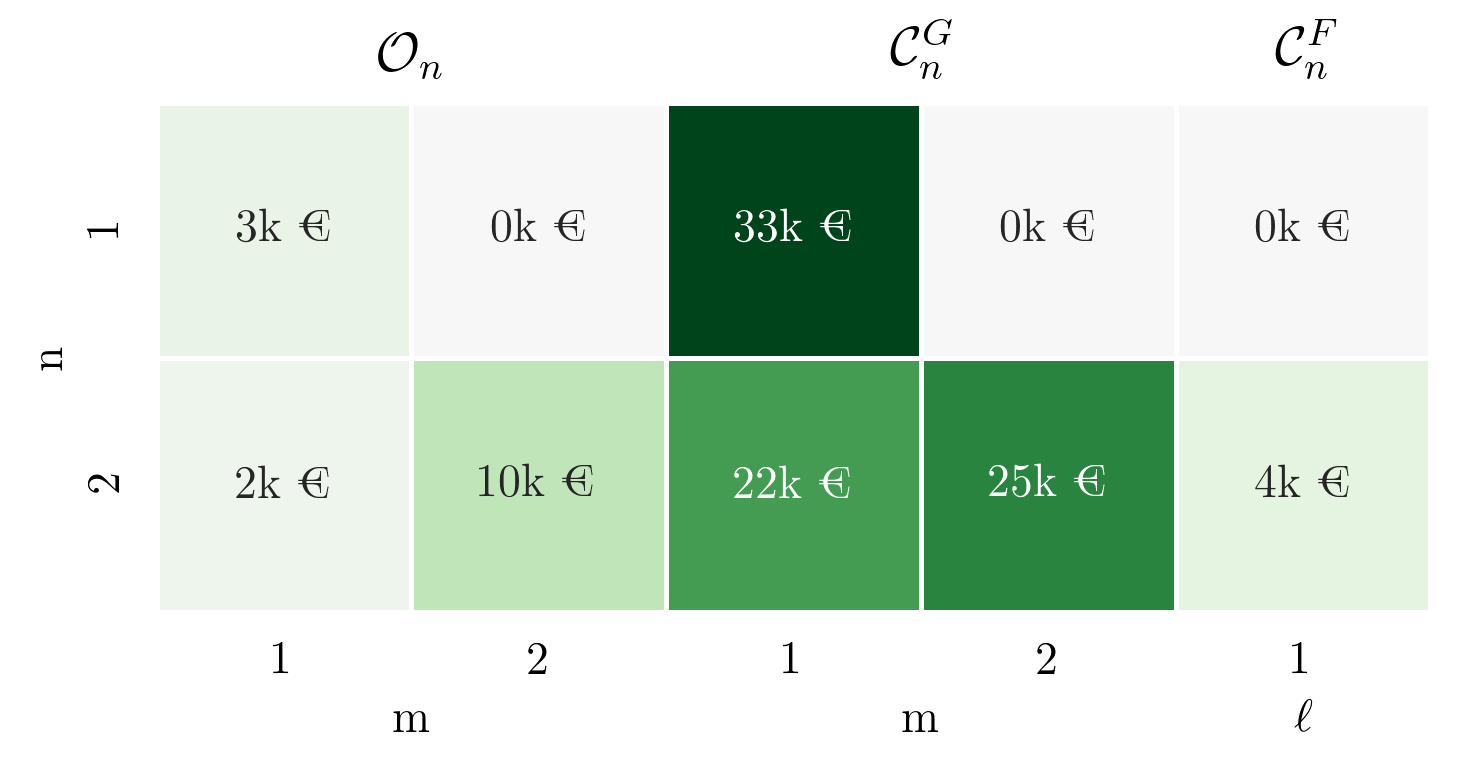
\includegraphics[width=\linewidth]{example_payoff_net_ebe.png}
    \caption{Full P2P cost allocation for the example setup shown in \cref{fig:example_network} when allocating net power injection using the EBE scheme (type \ref{net}\ref{ebe}). This leads to less and more intuitive payments.}
    \label{fig:example_payoff_net_ebe}
    \end{figure}    
% 
In contrast the to equivalent allocation of gross power production, netting out injections for each bus leads to less P2P payments. The resulting payment given in \cref{fig:example_payoff_net_ebe} builds on the allocated power flow shown \cref{fig:example_allocation_net_ebe} in \cref{sec:example_plots}. As bus~2 does not produce excess power, none of its power production is assigned to bus~1 and thus no payment of bus~1 to bus~2 allocated. Neither has bus~1 to pay fee to the transmission system as it only exports power. So, consumers at bus~1 pay to its local generator. Bus~2 in contrast bear all CAPEX for the transmission system as well as CAPEX and OPEX for generators at bus~1. 
% 
Again the cumulative payments per bus meet the nodal spending $\lmp \, \demand$. The cumulative revenues per generator and transmission line meet the all CAPEX and OPEX. Note this gives the same result as when allocating net injection with the Average Participation \ref{net}\ref{ap}.

The example shows that allocating net power injection only, reduces the number of peer-to-peer payments significantly, which leads to a much clearer pictures. The same counts for the AP scheme which we will use in the following application case.  

%We emphasize that the AP based allocation does not imply traceability of the resulting flows, as only the \textit{source}-\textit{sink} relations $\allocatepeer$ are determined by it, the flow allocation still follow the power plow equation given as shown in \cref{eq:allocate_peer_to_allocate_flow}.

\section{Application Case}

For showcasing the behavior of the cost allocation in a more complex system, we apply it to an cost-optimized German power system model with 50 nodes and one year time span with hourly resolution. The model builds on the PyPSA-EUR workflow \cite{horsch_jonas_pypsa-eur_2020} with technical details and assumptions reported in \cite{horsch_pypsa-eur_2018}. We follow a brownfield approach where transmission lines can be expanded starting from today's capacity values, originally retrieved from the ENTSO-E Transmission System Map \cite{entso-e_entso-e_nodate}. Pre-installed generation capacity totals for the year 2017 for wind and solar were distributed in proportion to the average power potential at each site excluding those with an average capacity factor of 10\%. Further, wind and solar capacity expansion are limited by land use restriction. These consider agriculture, urban, forested and protected areas based on the CORINE and NATURA2000 database \cite{corine2012,natura2000}. Pumped Hydro Storages (PHS) and Run-of-River power plants are fixed to today's capacities with no more expansion allowed. Additionally, unlimited expansion of batteries and H$_{2}$-storages and Open-Cycle Gas Turbines (OCGT) are allowed at each node. 
% 
\begin{figure*}[t]
    \centering
    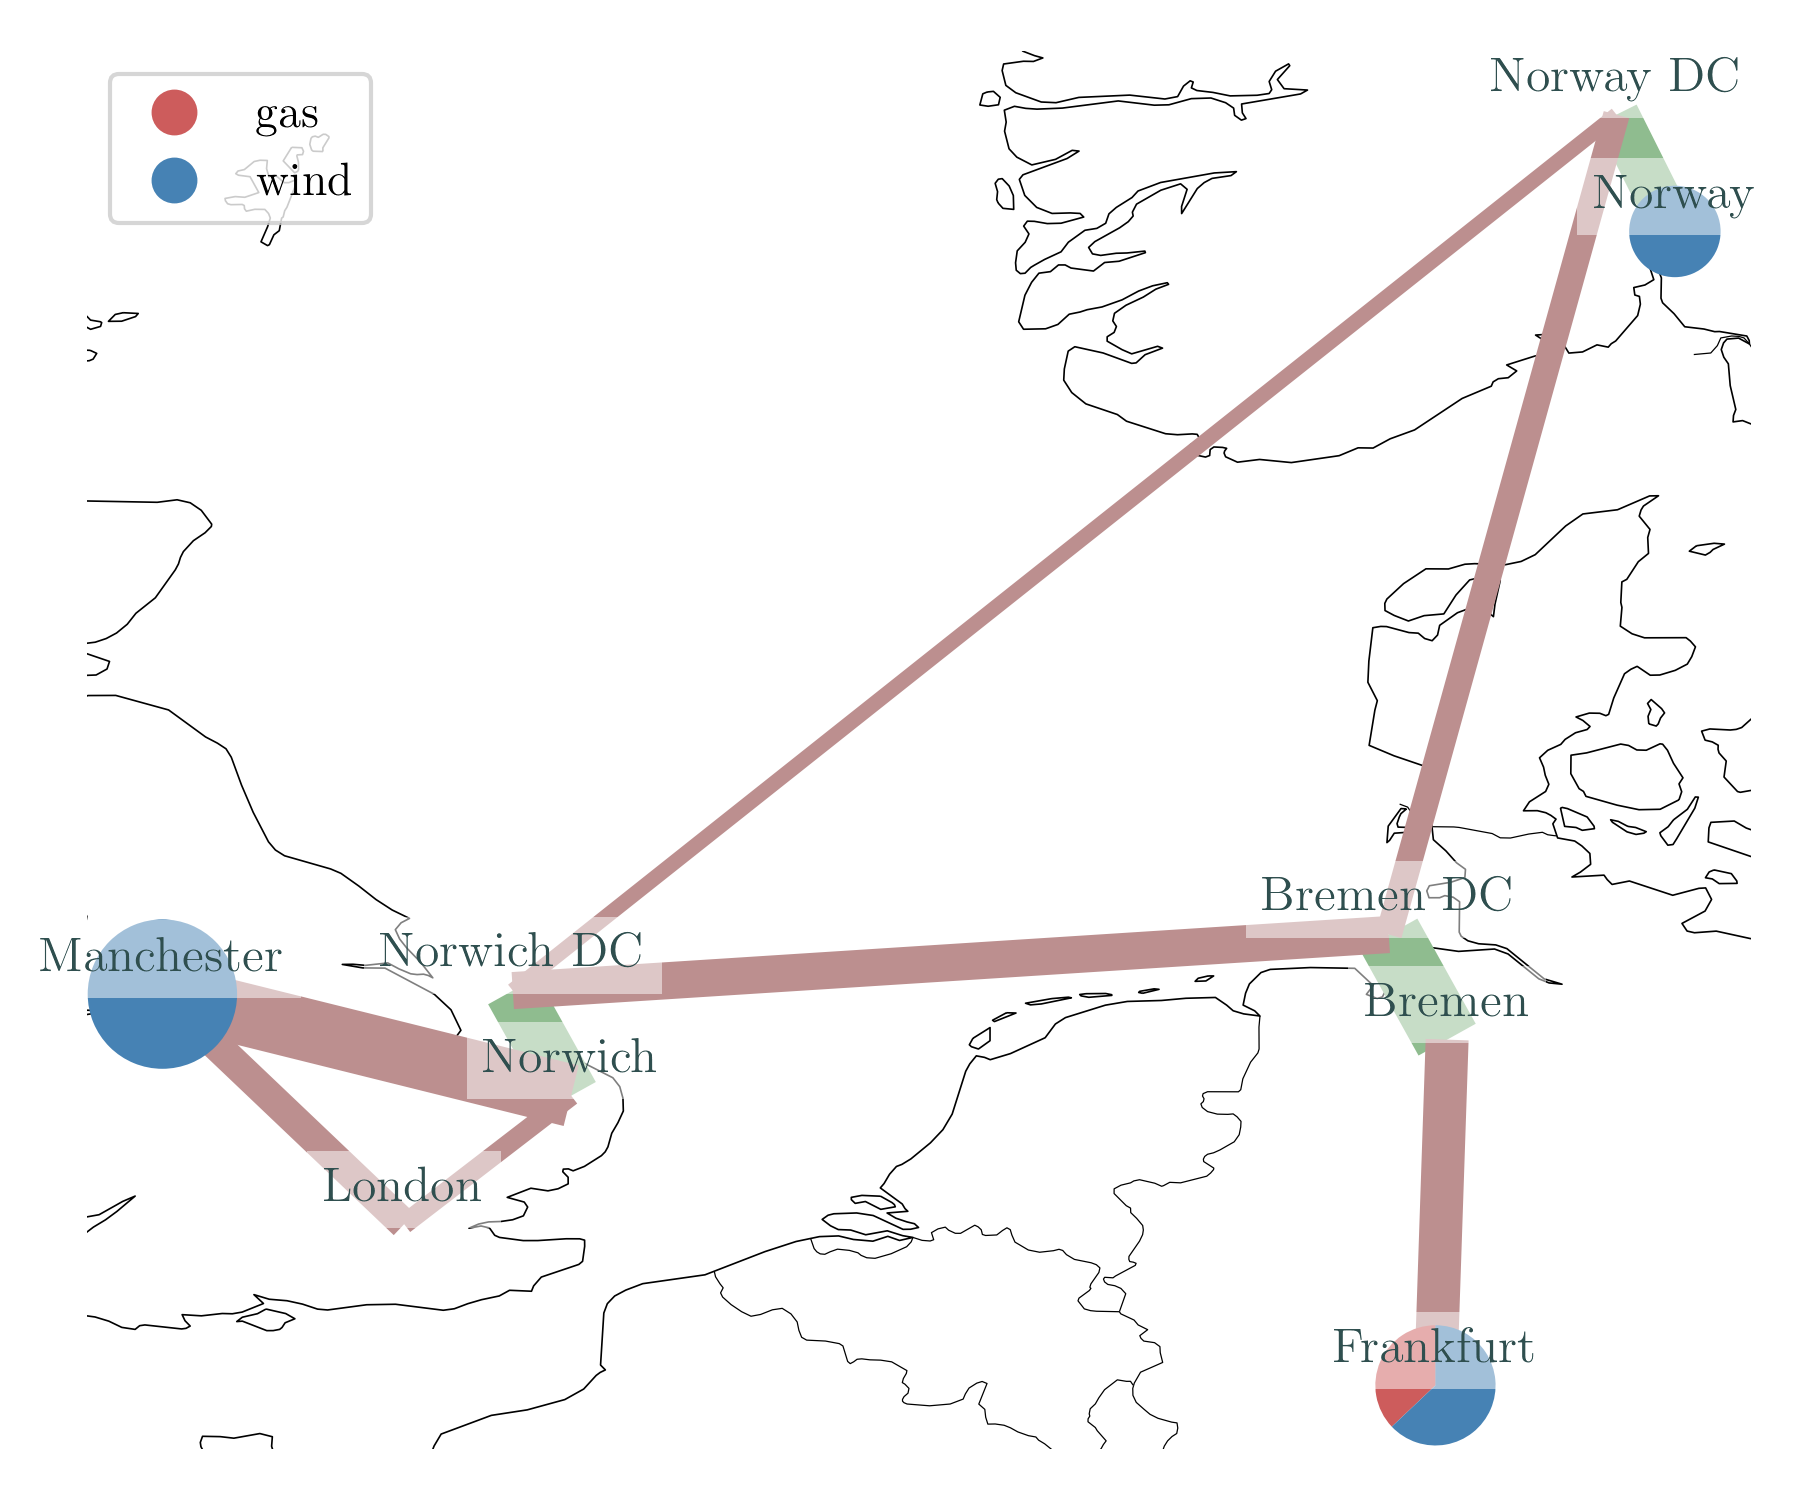
\includegraphics[width=\linewidth]{de50bf/network}
    \caption{Brownfield optimization of the German power system. The left side shows existent renewable capacities, matching the total capacity for the year 2017, which serve as lower capacity limits for the optimization. The right side shows the capacity expansion of renewables as well as installation of backup gas power plants. The effective CO$_2$ price is set to 120 \euro per tonne CO$_2$ emission.}
    \label{fig:network}
\end{figure*}
We impose a effective carbon price of 120 \euro\, per tonne-CO$_{2}$ which, with an gross emission of 180~kg/MWh and an efficiency of 39\% for OCGT, adds an price of 55 \euro/\megawatthour. All cost assumptions on operational costs $o_i$ and annualized capital cost $c_i$ are summarized in detail in \cref{tab:cost_assumptions}.
The optimized network is shown in  \cref{fig:network} with lower capacity bounds for renewable generators and transmission infrastructure on the left and capacity expansion for generation, storage and transmission on the right. The optimization expands the solar capacity in the south, onshore and offshore wind in the upper north and most west. Open-Cycle Gas Turbines (OCGT) are build within the broad middle of the network. Transmission lines are amplified in along the North-South axis, including one large DC link, associated with the German S\"ud-Link, leading from the coastal region to the South-West. 

\begin{figure}
    \centering
    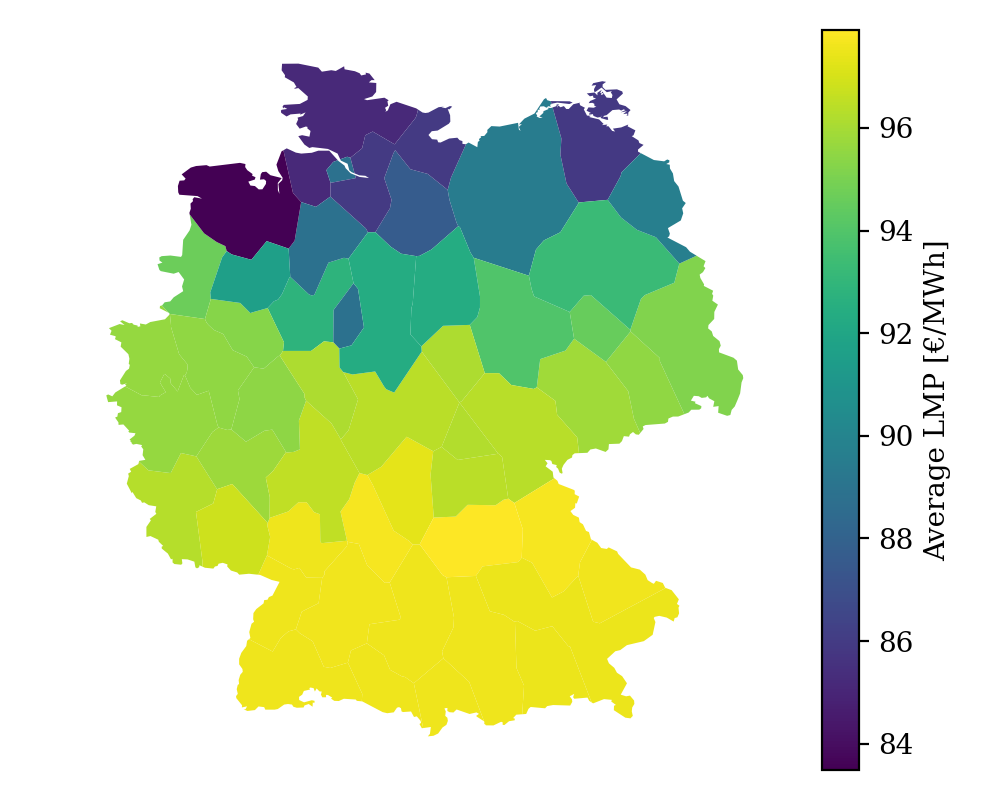
\includegraphics[width=\linewidth]{de50bf/average_price}
    \caption{Average electricity price $\lmp$ in the network.}
    \label{fig:average_price}
\end{figure}

The total annualized cost of the power system roughly sum up to 42 billion \euro.
\Cref{fig:average_price} displays the average electricity price $\lmp$ per region. We observe a relatively strong gradient from south (at roughly 92 \euro/MWh) to north (80 \euro/MWh). Regions with with little pre-installed capacity and capacity expansion, especially for renewables, tend to have higher prices. The node with the lowest LMP in the upper North-West, stands out through high pre-installed offshore capacities. \\


We allocate all costs under the assumtion that the \textit{net} dispatch is assigned according to the AP method (type \ref{net}\ref{ap}). This allocation suits the best for 
From the perspective of consumers, the largest proportion of the system cost is covered by payments associated with CAPEX for generators, transmission system and storage units in decreasing order, see \cref{fig:total_cost}. 
In \cref{fig:capex_price} we depict the regional distribution of the average price which consumers pay for a selection of different technologies. It turns out that  mostly areas with high CAPEX allocation are the ones with low average LMP. In particular, this counts for the coastal regions where strong offshore and onshore investments are taken. Inside the country, some regions also pay a fairly high shares dedicated to CAPEX, which are however allocated to non-local assets. The most even spatial distribution of CAPEX allocations accounts for OCGT. These are however primarily built nearby strong wind capacities.  

Together with the emission cost $\emissioncost$, the total OPEX $\opex$ amount around 16 billion \euro. As to expect, XX\% are dedicated to OCGT alone. In \cref{fig:opex_price,fig:emission_cost} we show the regional distribution of payments per MWh and the resulting revenues for generator...

The scarcity cost $\scarcitycost$, caused by land use constraints for renewables and the transmission expansion limit, sum up to roughly 7.5 b\euro. Note that according to \cref{eq:scarcitycost} this term is negative. It translates to  depicting the cost that consumers pay ``too much'' for assets limited in their capacity expansion. In the real world this money would be used to pay for augmented land costs in the dedicated areas. ...

The cost caused by lower capacity constraints for pre-existing assets which violate the optimal design are collected in $\subsidycost$. This ...

\begin{figure}
    \centering
    \includegraphics[width=0.75\linewidth]{de50bf/total_costs}
    \caption{Total allocated payments of the system. }
    \label{fig:total_cost}
\end{figure}




\begin{figure*}
    \centering
    \begin{subfigure}[c]{.6\linewidth}
    \includegraphics[width=\linewidth]{de50bf/ptpf_net_to_lowest-lmp}
    \end{subfigure}
    \hspace{-.2151\linewidth}
    \begin{subfigure}[c]{.6\linewidth}
    \includegraphics[width=\linewidth]{de50bf/ptpf_net_to_highest-lmp}
    \end{subfigure}
    \caption{Comparison of payments of the node with the \textbf{lowest LMP (left)} and the node with the \textbf{highest LMP (right)}. The region of the paying bus is colored in dark blue. The circles indicate where to which bus and technology combined OPEX and CAPEX payments. Further the thickness of the lines indicates the dedicated amount of payments. The cheap prices in the North...  }
    \label{fig:direct-allocation}
\end{figure*}









 
\begin{figure}
    \centering
    \includegraphics[width=\linewidth]{de50bf/locality_ptpf_net}
    \caption{Average distance between payer and receiver for different technologies and shares of the total production.}
    \label{fig:locality}
\end{figure}

\clearpage
\appendix

\section{Network Optimization}

\renewcommand\theequation{\thesection.\arabic{equation}}
\setcounter{equation}{0}

\renewcommand\thefigure{\thesection.\arabic{figure}}    
\setcounter{figure}{0}    

\subsection{LMP from Optimization}
The nodal balance constraint ensures that the amount of power that flows into a bus equals the power that flows out of a bus, thus reflects the Kirchhoff Current Law (KCL). Alternatively, we can the demand $\demand$ has to be supplied by the attached assets,  
\begin{align}
    \sum_i \incidenceasset \state  &=  \demand 
    % \sum_l \incidence \, \flow  - \nodalgeneration + \nodaldemand &= 0
     \resultsin{\lmp} \Forall{n,t}
    \label[constraint]{eq:nodal_balance_lin}
\end{align}
where $\incidenceasset$ is +1 if $i$ is attached to $n$ and a positive operation $\state$ delivers power to $n$, -1 if is attached to $n$ and a positive operation retrieves power from $n$ and zero else (note that for lines this results in the negative of the conventional Incidence Matrix).  
The shadow price of the nodal balance constraint mirrors the Locational Marginal Prizes (LMP) $\lmp$ per bus and time step. In a power market this is the \euro/\megawatthour-price which a consumer has to pay.\\

\subsection{Full Lagrangian}
\label{sec:full_lagrangian}
The Lagrangian for the investment model can be condensed to the following expression

\begin{align}
\notag
 \lagrangian\left(\state, \capacity, \lmp, \mu_j \right) =& 
 \;\;\; \sum_{i,t} o_i \state + \sum_{i} c_i \capacity  \\
\notag
&+  \sum_{n,t} \lmp \left( \demand - \sum_i \incidenceasset \, \state \right) \\
&+ \sum_j \mu_j \, h_j \left(\state, \capacity \right)
\label{eq:full_lagrangian}
\end{align}
where $h_j \left(\state, \capacity \right)$ denotes all inequality constraints attached to $\state$ and $\capacity$.
% \begin{align}
% \notag
% & \lagrangian\left(\generation, \flow, \capacitygeneration, \capacityflow, \boldsymbol{\lambda}, \boldsymbol{\mu} \right)   =   \\  
% \notag
% & \;\;\; \sum_{n,s} \capitalpricegeneration \capacitygeneration + \sum_{n, s, t} \operationalpricegeneration \generation + \sum_{\ell} \capitalpriceflow \, \capacityflow  \\
% \notag
% &+ \sum_{n,t} \lmp \left(\sum_\ell \incidence \, \flow  - \sum_s \incidencegenerator\, \generation +  \demand  \right)  \\ 
% \notag
% &+ \sum_{\ell,c,t} \cycleprice \, \cycle \, \impedance \, \flow  \\
% \notag
% &+ \sum_{n,s,t} \muuppergeneration \left( \generation - \generationpotential \capacitygeneration \right)  - \sum_{n,s,t} \mulowergeneration \generation  \\
% &+ \sum_{\ell,t} \muupperflow \left( \flow - \capacityflow \right) - \sum_{\ell,t} \mulowerflow \left( \flow + \capacityflow \right)     
% \label{eq:full_lagrangian}
% \end{align}
% 
% where $\boldsymbol{\lambda} = \left\lbrace \lmp, \cycleprice \right\rbrace $ and $\boldsymbol{\mu} = \left\lbrace \muuppergeneration, \mulowergeneration, \muupperflow, \mulowerflow \right\rbrace $ denote the set of related KKT variables. 
% 
In order to impose the Kirchhoff Voltage Law (KVL) for the linearized AC flow, the term 
\begin{align}
    \sum_{\ell,c,t} \cycleprice \, \cycle \, \impedance \, \flow 
\end{align}
can be added to $\lagrangian$, with $\impedance$ denoting the line's impedance and $\cycle$ being 1 if $\ell$ is part of the cycle $c$ and zero otherwise.

The global maximum of the Lagrangian requires stationarity with respect to all variables:
\begin{align}
    \pdv{\lagrangian}{\state} = \pdv{\lagrangian}{\capacity} = 0    
\end{align} 



\subsection{Zero Profit Generation}
\label{sec:zero_profit_generation}
\Cref{eq:upper_generation_capacity_constraint,eq:lower_generation_capacity_constraint}, which yield the KKT variables $\muuppergeneration$ and $\mulowergeneration$, imply the complementary slackness,
\begin{align}
\muuppergeneration \left( \generation - \generationpotential \, \capacitygeneration \right)  &= 0  \Forall{n,s,t} 
\label{eq:complementary_slackness_upper_generation} \\
\mulowergeneration  \, \generation &= 0 \Forall{n,s,t}
\label{eq:complementary_slackness_lower_generation} 
\end{align}


The stationarity of the generation capacity variable leads to 
\begin{align}
\pdv{\lagrangian}{\capacitygeneration}  = 0 \,\, \rightarrow \,\, 
\capitalpricegeneration =  \sum_t \muuppergeneration \, \generationpotential  \Forall{n,s}
\label{eq:capex_generation_duality}
\end{align}
and the stationarity of the generation to 
\begin{align}
\pdv{\lagrangian}{\generation} &= 0 \,\, \rightarrow \,\,  
\operationalpricegeneration =  \incidencegenerator \, \lmp - \muuppergeneration + \mulowergeneration \Forall{n,s} \label{eq:opex_duality}
\end{align}


Multiplying both sides of \cref{eq:capex_generation_duality} with $\capacitygeneration$ and using \cref{eq:complementary_slackness_upper_generation} leads to 
\begin{align}
 \capitalpricegeneration \, \capacitygeneration  = \sum_t \muuppergeneration \, \generation 
 \label{eq:capital_price_generation_sum}
\end{align}
The zero-profit rule for generators is obtained by multiplying \cref{eq:opex_duality} with $\generation$ and using \cref{eq:complementary_slackness_lower_generation,eq:capital_price_generation_sum} which results in 
\begin{align}
  \capitalpricegeneration \, \capacitygeneration + \sum_t \operationalpricegeneration \generation = \sum_t \lmp \incidencegenerator \generation
\end{align}
It states that over the whole time span, all OPEX and CAPEX for generator $s$ (left hand side) are payed back by its revenue (right hand side).

\subsection{Zero Profit Transmission System}
\label{sec:zero_profit_flow}

The yielding KKT variables $\muupperflow$ and $\mulowerflow$ are only non-zero if $\flow$ is limited by the transmission capacity in positive or negative direction, i.e. \cref{eq:upper_flow_capacity_constraint} or \cref{eq:lower_flow_capacity_constraint} are binding. For flows below the thermal limit, the complementary slackness 
\begin{align}
\muupperflow \left( \flow - \capacityflow \right)  &= 0 \Forall{\ell,t}
\label{eq:complementary_slackness_upper_flow} \\
\mulowerflow \left( \flow - \capacityflow \right) &=  0 \Forall{\ell,t}
\label{eq:complementary_slackness_lower_flow} 
\end{align}
sets the respective KKT to zero. 

The stationarity of the transmission capacity to
\begin{align}
\pdv{\lagrangian}{\capacityflow} = 0 \,\, \rightarrow \,\, 
\capitalpriceflow =  \sum_t \left( \muupperflow - \mulowerflow \right) \Forall{\ell}
\label{eq:capexFlow_duality}
\end{align}
and the stationarity with respect to the flow to
\begin{align}
    0 &= \pdv{\lagrangian}{\flow}  \\ 
    0 &= - \sum_n \incidence \lmp  + \cycleprice \cycle \impedance  - \muupperflow + \mulowerflow \Forall{n,s} \label{eq:opex_flow_duality}
\end{align}
    
    
When multiplying \cref{eq:capexFlow_duality} with $\capacityflow$ and using the complementary slackness \cref{eq:complementary_slackness_upper_flow,eq:complementary_slackness_lower_flow} we obtain 
\begin{align}
 \capitalpriceflow \, \capacityflow = \sum_t \left( \muupperflow - \mulowerflow \right)  \, \flow
 \label{eq:capital_price_flow_sum}
\end{align}
Again we can use this to formulate the zero-profit rule for transmission lines. We multiply \cref{eq:opex_flow_duality} with $\flow$, which finally leads us to 
\begin{align}
\capitalpriceflow \, \capacityflow = - \sum_n \incidence\, \lmp\, \flow + \cycleprice\, \cycle\, \impedance\, \flow 
\end{align}
% Watch out Incidence = - ordinary Incidence !!
It states that the congestion revenue of a line (first term right hand side) reduced by the cost for cycle constraint exactly matches its CAPEX. 


\subsection{Zero Profit Storage Units}
\label{sec:zero_profit_storage_units}

For an simplified storage model, the upper capacity $\capacitystorage$ limits the discharging dispatch $\storagedispatch$, the storing power $\storagecharge$ and state of charge $\storagesoc$ of a storage unit $r$ by 
\begin{align}
    \storagedispatch - \capacitystorage &\le 0 \Forall{r,t} \resultsin{\muupperstoragedispatch} \\
    \storagecharge - \capacitystorage &\le 0 \Forall{r,t} \resultsin{\muupperstoragecharge} \\
    \storagesoc - h_r \, \capacitystorage &\le 0 \Forall{r,t} \resultsin{\muupperstoragesoc}
\end{align}
where we assume a fixed ratio between dispatch and storage capacity of $h_r$. 
% From stationarity we obtain 
% \begin{align}
%     \notag
%     \pdv{\lagrangian}{\capacitystorage} &= 0 \\
%     \capitalpricestorage &= \sum_t \left( \muupperstoragedispatch + \muupperstoragecharge + h_r \muupperstoragesoc  \right)
% \end{align}
The state of charge must be consistent throughout every time step according to what is dispatched and stored, 
\begin{align}
    \notag
    \storagesoc - \efficiencysoc \storageprevioussoc - \efficiencycharge \storagecharge &+ (\efficiencydispatch)^{-1} \storagedispatch = 0 \\
    &\resultsin{\mustateofcharge} \Forall{r,t}
\end{align}



We use the result of Appendix B.3 in \cite{brown_decreasing_2020} which shows that a storage recovers its capital (and operational) costs from aligning dispatch and charging to the LMP, thus 
\begin{align}
    \sum_t \operationalpricestorage \, \storagedispatch + \capitalpricestorage \, \capacitystorage = \sum_t \lmp \incidencestorage \left(\storagedispatch - \storagecharge \right) 
\end{align}
The stationarity of the dispatched power leads us to  
\begin{align}
    \notag
    \pdv{\lagrangian}{\storagedispatch} &= 0 \\
    \operationalpricestorage -  \lmp \, \incidencestorage - \mulowerstoragedispatch + \muupperstoragedispatch + (\efficiencydispatch )^{-1} \mustateofcharge &= 0  
    \label{eq:stationarity_storagedispatch}
\end{align}
which we  can use to define the revenue which compensates the CAPEX at $r$, 
\begin{align}
    \notag
    \capitalpricestorage \, \capacitystorage = \sum_t \left(\muupperstoragedispatch - \mulowerstoragedispatch  + (\efficiencydispatch )^{-1} \mustateofcharge \right) \storagedispatch \\
    - \sum_t \lmp \incidencestorage  \storagecharge \Forall{r} 
\end{align}

% With this constraint we can derive the following stationarities:
% \begin{align}
%     \notag
%     \pdv{\lagrangian}{\storagedispatch} &= 0 \\
%     \operationalpricestorage + \lmp + \mulowerstoragedispatch - \muupperstoragedispatch - (\efficiencydispatch )^{-1} \mustateofcharge &= 0  
%     \label{eq:stationarity_storagedispatch}
% \end{align}
% \begin{align}
%     \notag
%     \pdv{\lagrangian}{\storagecharge} &= 0 \\
%     - \lmp + \mulowerstoragecharge - \muupperstoragecharge + \efficiencycharge \mustateofcharge &= 0 
%     \label{eq:stationarity_storagecharge}
% \end{align}
% \begin{align}
%     \notag
%     \pdv{\lagrangian}{\storagesoc} &= 0 \\
%     \mulowerstoragesoc - \muupperstoragesoc - \mustateofcharge + \efficiencysoc \munextstateofcharge &= 0 
%     \label{eq:stationarity_storagesoc}
% \end{align}



\subsection{Emission Constraint}

Imposing an additional CO$_2$ constraint limiting the total emission to K,  
\begin{align}
\sum_{n,s,t} \emission \, \generation \le \text{K} \resultsin{\emissionprice} 
\label[constraint]{eq:co2_constraint}
\end{align}
with $\emission$ being the emission factor in tonne-CO$_2$ per \megawatthour, returns an effective CO$_2$ price $\emissionprice$ in \euro/tonne-CO$_2$. 
% The CO$_2$ price shifts the right hand side of the non-profit relation for generators \cref{eq:non_profit_generator} to
% 
% \begin{align}
% \capitalpricegeneration \, \capacitygeneration + \sum_{t} \operationalpricegeneration \, \generation &= \sum_{t} \left( \lmp - \emission \, \emissionprice \right)  \, \generation \Forall{n,s} 
% \label{eq:non_profit_generator_emission}
% \end{align}
% This shows nicely the duality for exchanging the CO$_2$ \cref{eq:co2_constraint} for a shifted OPEX which includes the CO$_2$ costs
As shown in ... the constraint can be translated in a dual price which shift the operational price per generator
\begin{align}
\operationalpricegeneration \rightarrow \operationalpricegeneration + \emission \, \emissionprice \label[relation]{eq:shift_opex_by_emission_cost}
\end{align}



% \subsection{Brownfield Optimization and Capacity Restrictions}

% Constraining the capacities $\capacitygeneration$  for a subset $S$ of generators to lower or upper limits in the form of
% \begin{align}
%     \capacitygenerationlower - \capacitygeneration \le 0 \resultsin{\mulowergenerationnom} \hpad \forall{s \in S} \label{eq:capacityexpansionminimum}\\
%     \capacitygeneration - \capacitygenerationupper \le 0 \resultsin{\muuppergenerationnom} \hpad \forall{s \in S}
% \label{eq:capacityexpansionmaximum}
% \end{align}
% alters the objective value as soon as one of those become bounding. 
% The complementary slackness for both are 
% \begin{align}
%     \muuppergenerationnom \left( \capacitygeneration - \capacitygenerationupper \right) =0 \Forall{s \in S} \\
%     \mulowergenerationnom \left( \capacitygeneration - \capacitygenerationlower \right) =0 \Forall{s \in S}
% \end{align}


% The CAPEX paybacks for generators and transmission lines
% \cref{eq:capital_price_generation_sum,eq:capital_price_flow_sum} change to 
% \begin{align}
% \pdv{\lagrangian}{\capacitygeneration}  = 0 \,\, \rightarrow \,\, \\
% \capitalpricegeneration =  \sum_t \muuppergeneration \, \generationpotential + \mulowergenerationnom - \muuppergenerationnom \Forall{s \in S}
% \label{eq:capex_generation_duality_bf}
% \end{align}
% for generators. Multiplying \cref{eq:capex_generation_duality_bf} by $ \capacitygeneration$ leads us to 
% \begin{align}
%  \capexgeneration_s - \remainingcost_s=  \sum_t \muuppergeneration \, \generation \Forall{n,s \in S}
%  \label{eq:capex_generation_duality_bf2}
% \end{align}
% where we define the cost resulting from the capacity expansion limits as
% \begin{align}
%     \remainingcost_s = \left(\mulowergenerationnom - \muuppergenerationnom \right) \capacitygeneration
%     \Forall{s}
% \end{align}
% As $\mulowergenerationnom \ge 0$ and $\muuppergenerationnom \ge 0$, the latter can be a net positive or net negative cost term.

% Multiplying \cref{eq:opex_duality}, which is still valid, with $\generation$ and inserting \cref{eq:capex_generation_duality_bf2} will bring us to the zero profit rule for generators with capacity expansion limits, 
% \begin{align}
%     \capexgeneration_s + \opexgeneration_s  - \remainingcost_s = \sum_t \lmp \incidencegenerator \generation \Forall{s \in S}
% \end{align}
% We see that the revenue of generator $s$ will not exactly pay back its full CAPEX and OPEX. The exogenous constraint shifts the zero-profit equations such that some of the expenditures for $s \in S$ cannot directly be allocated to consumers. In order to take this effect into account for the cost allocation, we update the shadow price $\muuppergeneration$ in \cref{tab:cost_allocation_map}, to 

% \begin{align}
%     \muuppergeneration \rightarrow \dfrac{\capitalpricegeneration}{\capitalpricegeneration - \mulowergenerationnom + \muuppergenerationnom}\, \muuppergeneration
% \end{align}
% By doing so we ensure that the allocated CAPEX sum up to the actual CAPEX at generator $s$, thus 
% \begin{align}
%     \capexgeneration_s = \sum_{n,t} \allocatecapexgeneration \Forall{s \in S}
% \end{align}



% Doing likewise with a subset $L$ of transmission lines,
% \begin{align}
% \capacityflow \ge \capacityflowLower \resultsin{\mulowerflownom} \hpad \forall{\ell \in \textit{L}} \\
% \capacityflow \le \capacityflowUpper \resultsin{\muupperflownom} \hpad \forall{\ell \in \textit{L}}
% \end{align}
% results in a shifted zero-profit rule for transmission line in the form 
% \begin{align}
%     \capitalpriceflow \, \capacityflow - \remainingcost_\ell = \sum_{n,t}\allocatecapexflow \Forall{\ell \in L}
% \end{align}
% where $\remainingcost_\ell$ is given by 
% \begin{align}
%     \remainingcost_\ell = \left(\mulowerflownom - \muupperflownom \right) \, \capacityflow
%     \Forall{\ell \in L}
% \end{align}

% % \begin{align}
% %     \muupperflownom \left( \capacityflow - \capacityflowUpper \right) =0 \\
% %     \mulowerflownom \left( \capacityflow - \capacityflowLower \right) =0 \\
% % \end{align}

% % \begin{align}
% %     \pdv{\lagrangian}{\capacityflow}  = 0 \,\, \rightarrow \,\, \\
% %     \capitalpriceflow =  \sum_t \left( \muupperflow - \mulowerflow \right)  + \mulowerflownom - \muupperflownom \Forall{n,s}
% %     \label{eq:capex_flow_duality_bf}
% %     \end{align}
% %     for transmission lines.
% % Multiplying \cref{eq:capex_generation_duality_bf} by the amount of expansion $\left( \capacitygeneration - \capacitygenerationlower \right) $
% % \begin{align}
% %   \capitalpricegeneration \, \capacitygeneration^{exp} =  \sum_t \muuppergeneration \, \left( \generation - \generationpotential \, \capacitygenerationlower \right) + \muuppergenerationnom \left( \capacitygenerationupper - \capacitygenerationlower \right) \Forall{n,s}
% % \end{align}






\section{Allocation Schemes}
\subsection{Allocating Gross Injections with EBE}
\label{sec:gross_ebe}

The allocation of gross generation to demands $\demand$ is straightforwardly obtained by a proportional distribution of the generation, \ie

\begin{align}
    \allocategeneration = \dfrac{\generation}{\sum_s \generation} \demand 
\end{align}


\subsection{Allocating Net Injections with EBE}
\label{sec:net_ebe}

Allocating net power injections using the EBE methods leads to the same result as the Marginal Participation (MP) \cite{rudnick_marginal_1995}  algorithm when allocating to consumers only, see \cite{hofmann_flow_2020-1} for further insight. We calculate it by setting 
\begin{align}
\allocatepeer &=  \delta_{m,n}\,\selfconsumption[m] + \gamma_t \, \netconsumption  \, \netproduction[m]
\label{eq:mp_slack}
\end{align}
where 
\begin{itemize}
%  \item $\injection = \left( \nodalgeneration - \nodaldemand \right) $ denotes the nodal injection
\item $\netproduction = \text{min}\left( \nodalgeneration - \nodaldemand , 0 \right) $ denotes the nodal net production 
\item $\netconsumption = \text{min}\left( \nodaldemand  - \nodalgeneration, 0 \right)$ denotes the nodal net consumption
\item $\selfconsumption = \text{min}\left( \netproduction, \netconsumption \right)$ the denotes  nodal self-consumption. That is the power generated and at the same time consumed at node $n$ and 
\item $\gamma_t = \left( \sum_n \netproduction\right) ^{-1} = \left( \sum_n \netconsumption\right) ^{-1}$ is the inverse of the total injected/extracted power at time $t$.
\end{itemize}

The allocation $\allocategeneration$ from generator $s$ to $n$, is given by multiplying $\allocatepeer$ with the nodal share $\generation / \nodalgeneration$.


\subsection{Allocating Net Power using AP}
\label{sec:net_ap}

\newcommand{\incidenceM}{K}
\newcommand{\flowM}{f}
\newcommand{\injectionM}{p}
\newcommand{\slackM}{k}
\newcommand{\DirectedIncidence}{\mathcal{K}}
\newcommand{\InverseAPInjection}{\mathcal{J}}
\newcommand\diag[1]{\operatorname{diag}\left(#1\right)}


Allocating net injections using the AP method is derived from \cite{achayuthakan_electricity_2010}. In a lossless network the downstream and upstream formulations result in the same P2P allocation which is why we restrict ourselves to the downstream formulation only. In a first step we define a time-dependent auxiliary matrix $\InverseAPInjection_t$ which is the inverse of the $N\times N$ with directed power flow $m \rightarrow n$ at entry $(m, n)$ for $m \ne n$ and the total flow passing node $m$ at entry $\left( m, m\right)$ at time step $t$. Mathematically this translates to


\begin{align}
\InverseAPInjection_t = \left( \diag{\injectionM^+} + \DirectedIncidence^- \diag{\flowM} \, \incidenceM \right)_t^{-1} 
\end{align}
where $\DirectedIncidence^-$ is the negative part of the directed Incidence matrix $\DirectedIncidence_{n,\ell} = \text{sign}\left( \flow \right)  \incidence$. Then the distributed slack for time step $t$ is given by
\begin{align}
\allocatepeer = \InverseAPInjection_{m,n,t} \, \netproduction[m] \, \netconsumption
\end{align}

\subsection{Allocating Gross Power using AP}
\label{sec:gross_ap}

We use the same allocation as in \cref{sec:net_ap} but replace the net nodal production $\netproduction$ by the gross nodal production $\nodalgeneration$ which leads to  
\begin{align}
\InverseAPInjection_t = \left( \diag{g} + \DirectedIncidence^- \diag{\flowM} \, \incidenceM \right)_t^{-1} 
\end{align}
The distributed slack is for time step $t$ is then given by
\begin{align}
\allocategeneration[s \rightarrow m] = \InverseAPInjection_{m,n} \, \generation \, \demand
\end{align}


\subsection{Numerical Example: Power Flow Allocation of type \ref{net}\ref{ebe}}
\label{sec:example_plots}
\begin{figure}[h!]
    \begin{subfigure}[c]{.99\linewidth}
    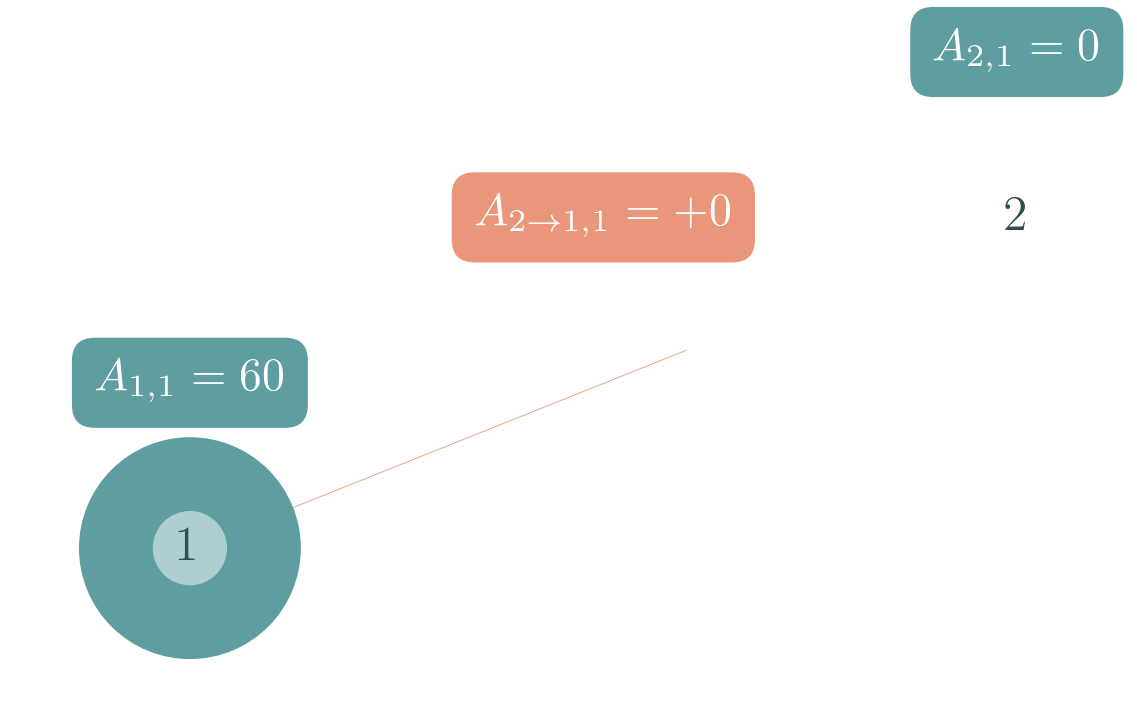
\includegraphics[width=\linewidth]{example_allocation_bus1_net_ebe.png}
    \vspace{-40pt}
    \subcaption{}
    \label{fig:example_allocation_bus1_net_ebe}
    \end{subfigure}
    \begin{subfigure}[c]{.99\linewidth}
    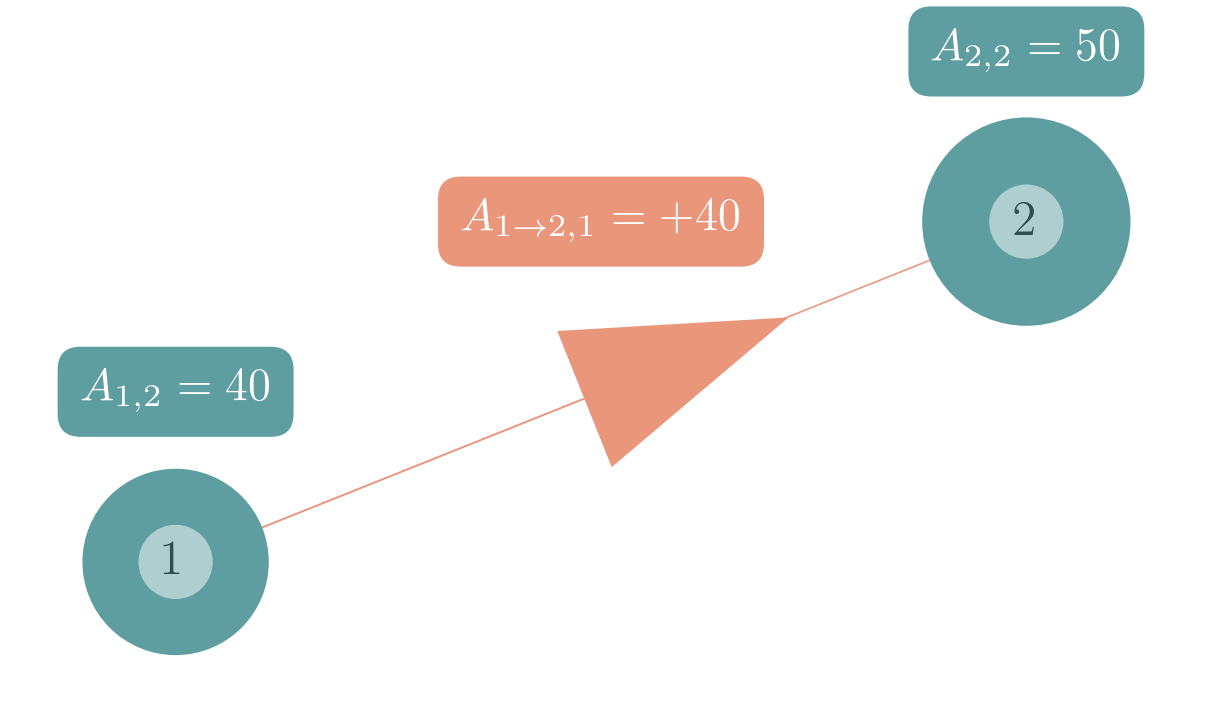
\includegraphics[width=\linewidth]{example_allocation_bus2_net_ebe.png}
    \vspace{-40pt}
    \subcaption{}
    \label{fig:example_allocation_bus2_net_ebe}
    \end{subfigure}
    \caption{Power allocations for bus~1 (a) and bus~2 (b) of the example network in \cref{fig:example_network} using equivalently allocated net power injections (scheme \ref{net}\ref{ebe}). Bus~1 retrieves 60~MW from itself and nothing from bus~2. The latter in turn retrieves 40~MW from bus~1 and self supplies 50~MW. The P2P trades are less in number and more intuitive then with allocating gross flow.}
    \label{fig:example_allocation_net_ebe}
\end{figure}
% 
\section{Working Example}
The following figures contain more detailed information about the peer-to-peer cost allocation. The cost or prices payed by consumers are indicated by the region color. The dedicated revenue is displayed in proportion to the size of cycles (for assets attached to buses) or to the thickness of transmission branches.    
\begin{figure*}
    \centering
    \begin{subfigure}[c]{.49\linewidth}
        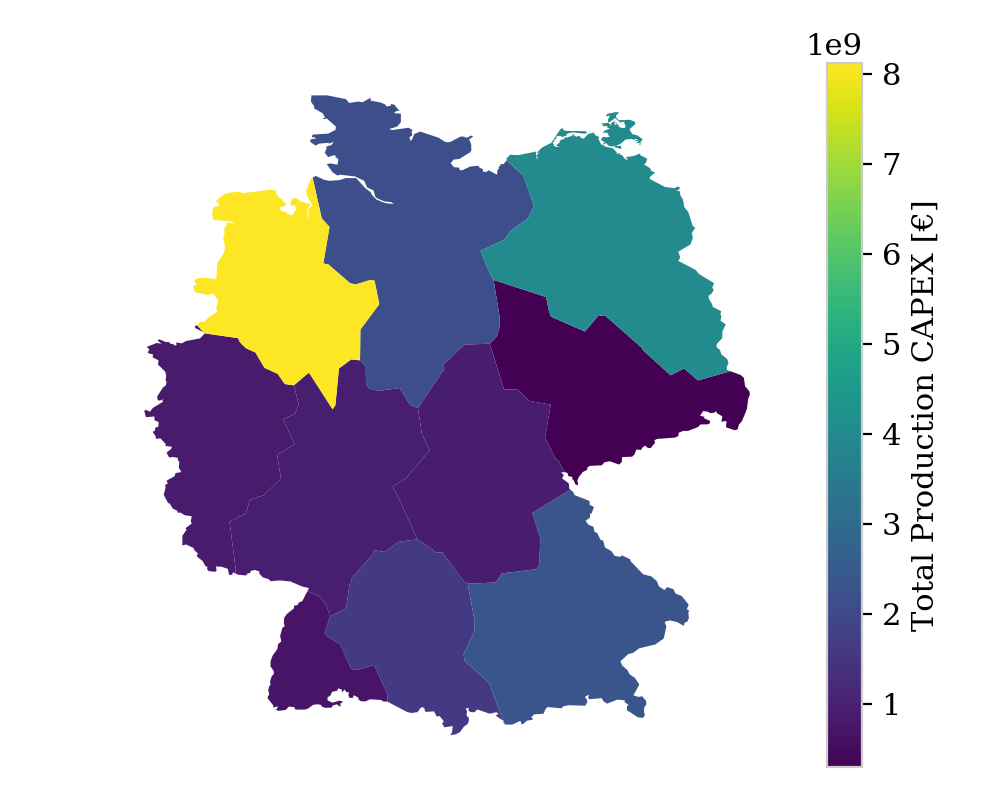
\includegraphics[width=\linewidth]{de50bf/maps_price_ptpf_net/one_port_investment_cost_total}
        \subcaption{All production and storage technologies}
        \label{fig:total_capex}
    \end{subfigure}
    \begin{subfigure}[c]{.49\linewidth}
        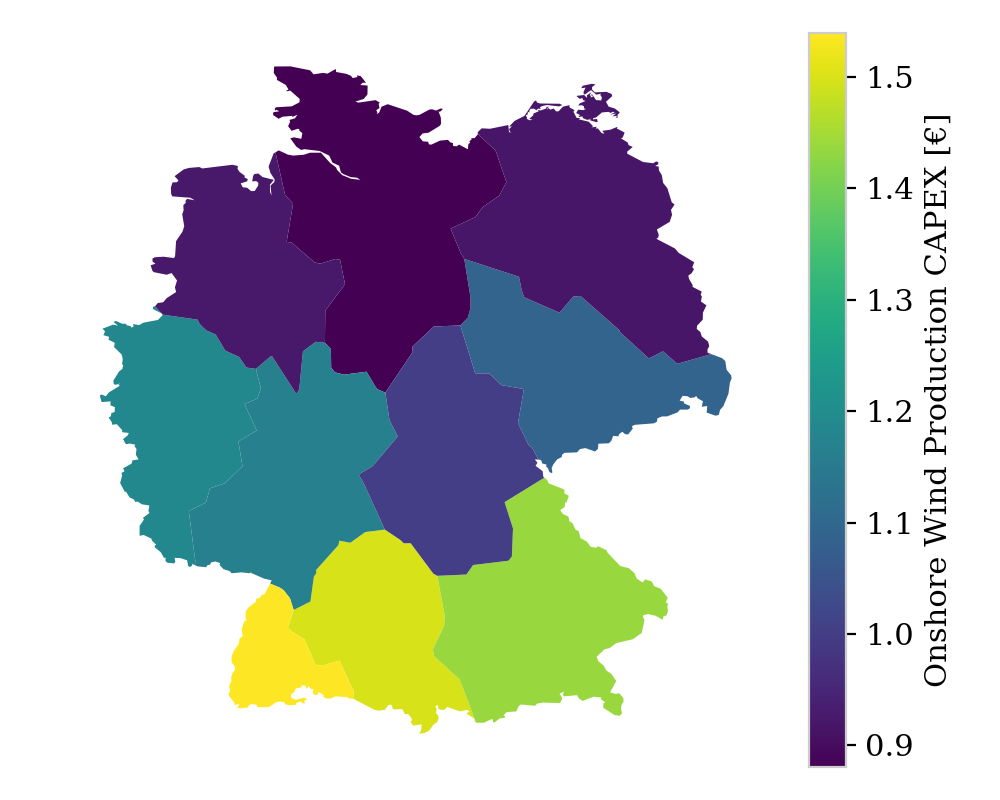
\includegraphics[width=\linewidth]{de50bf/maps_price_ptpf_net/by_carrier/onwind_one_port_investment_cost}
        \subcaption{Onshore Wind}
        \label{fig:onshore_capex}
    \end{subfigure}
    \begin{subfigure}[c]{.49\linewidth}
        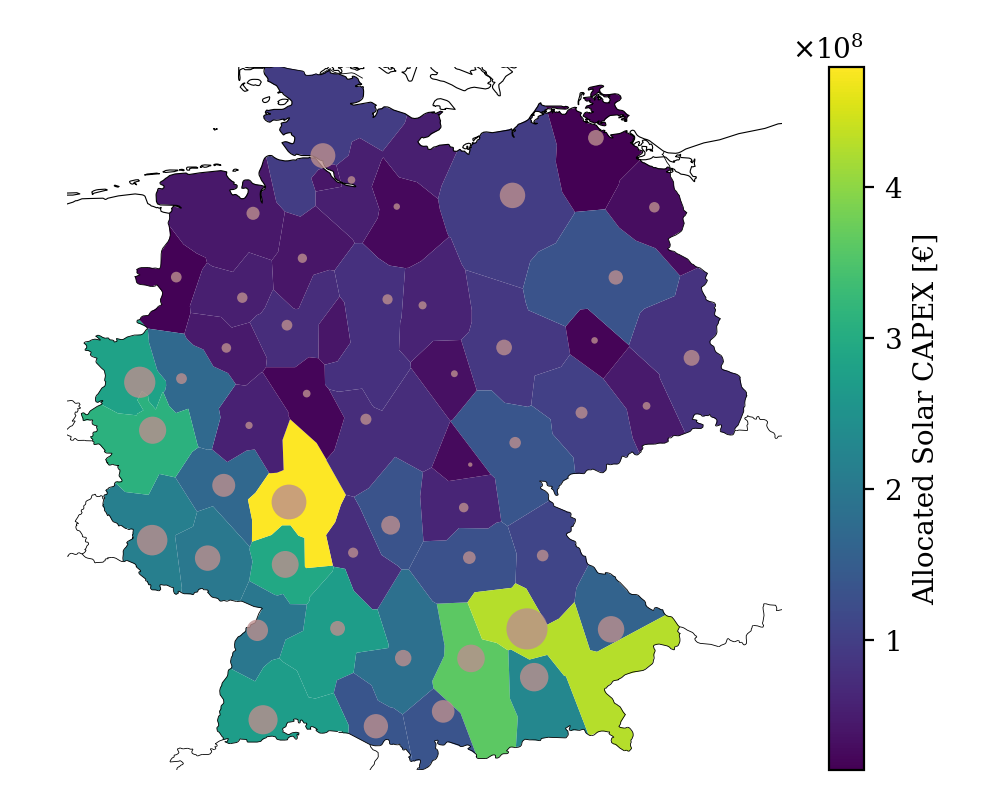
\includegraphics[width=\linewidth]{de50bf/maps_price_ptpf_net/by_carrier/solar_one_port_investment_cost}
        \subcaption{Solar}
        \label{fig:solar_capex}
    \end{subfigure}
    \begin{subfigure}[c]{.49\linewidth}
        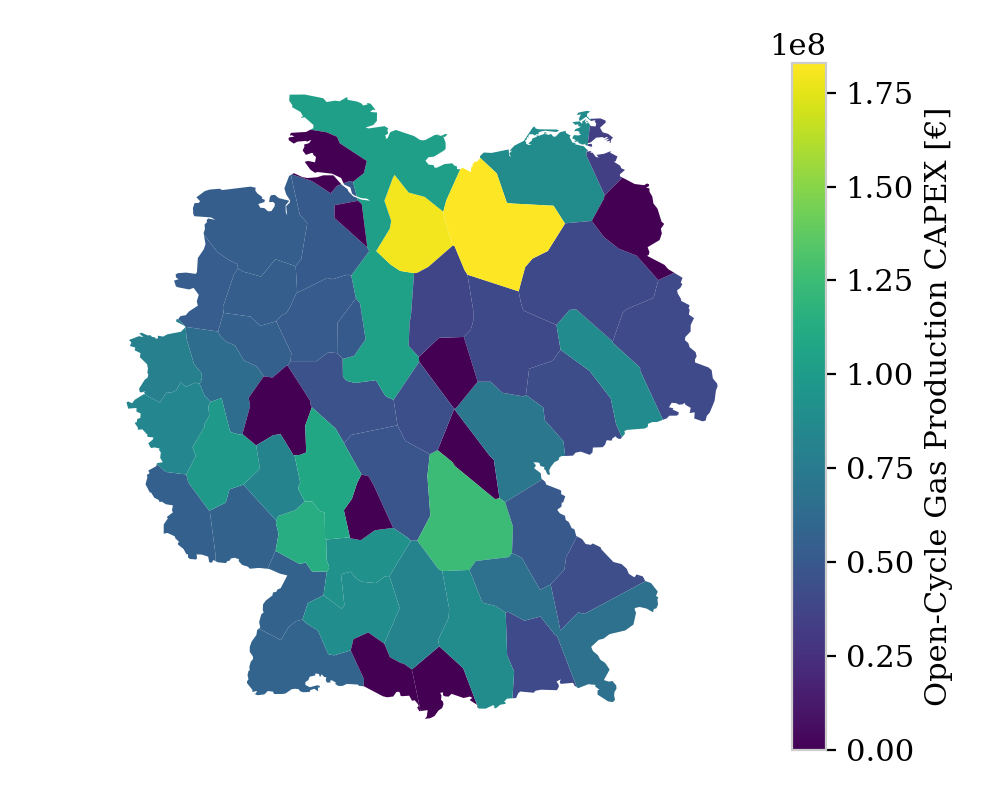
\includegraphics[width=\linewidth]{de50bf/maps_price_ptpf_net/by_carrier/OCGT_one_port_investment_cost}
        \subcaption{OCGT}
        \label{fig:ocgt_capex}
    \end{subfigure}
    \caption{Average electricity price due to \textbf{CAPEX allocation}, $\sum_t \allocatecapexgeneration$ and $\sum_t \allocatecapexstorage$, for all assets, onshore wind, solar and OCGT. Average Allocated CAPEX per MWh within the regions are indicated by the color, the revenue per production asset is given by the size of the circles at the corresponding bus.}
    \label{fig:capex_price}
\end{figure*}

\begin{table*}[h]
    \centering
    \begin{tabular}{lllr}
\toprule
     &    & o [\euro/MWh] &  c [k\,\euro/MW]$^*$ \\
{} & carrier &               &                      \\
\midrule
Generator & Open-Cycle Gas &       120.718 &               47.235 \\
     & Offshore Wind (AC) &         0.015 &              203.116 \\
     & Offshore Wind (DC) &         0.015 &              230.532 \\
     & Onshore Wind &         0.015 &              109.296 \\
     & Run of river &               &              270.941 \\
     & Solar &          0.01 &               55.064 \\
Storage & Hydrogen Storage &               &              224.739 \\
     & Pumped Hydro &               &              160.627 \\
     & Battery Storage &               &              133.775 \\
Line & AC &               &                0.038 \\
     & DC &               &                0.038 \\
\bottomrule
\end{tabular}
    
    \caption{Operational and capital price assumptions for all type of assets used in the working example. The capital price for transmission lines are given in [k\,\euro/MW/km]. The cost assumptions are retrieved from the PyPSA-EUR model \cite{horsch_jonas_pypsa-eur_2020}.}
    \label{tab:cost_assumptions}
\end{table*} 

\begin{figure}
    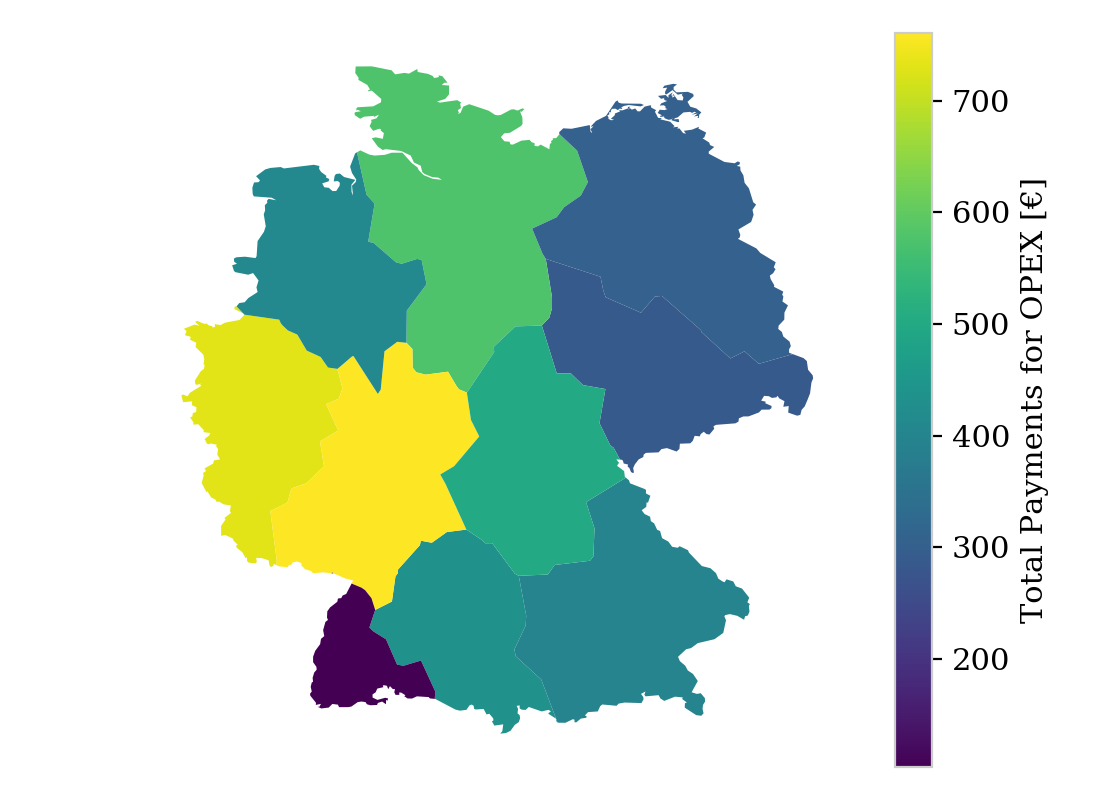
\includegraphics[width=\linewidth]{de50bf/maps_price_ptpf_net/one_port_operational_cost_total}
    \caption{Average electricity price \textbf{OPEX allocation}, $\sum_t \allocateopex$.}
    \label{fig:opex_price}
\end{figure}


\begin{figure}
    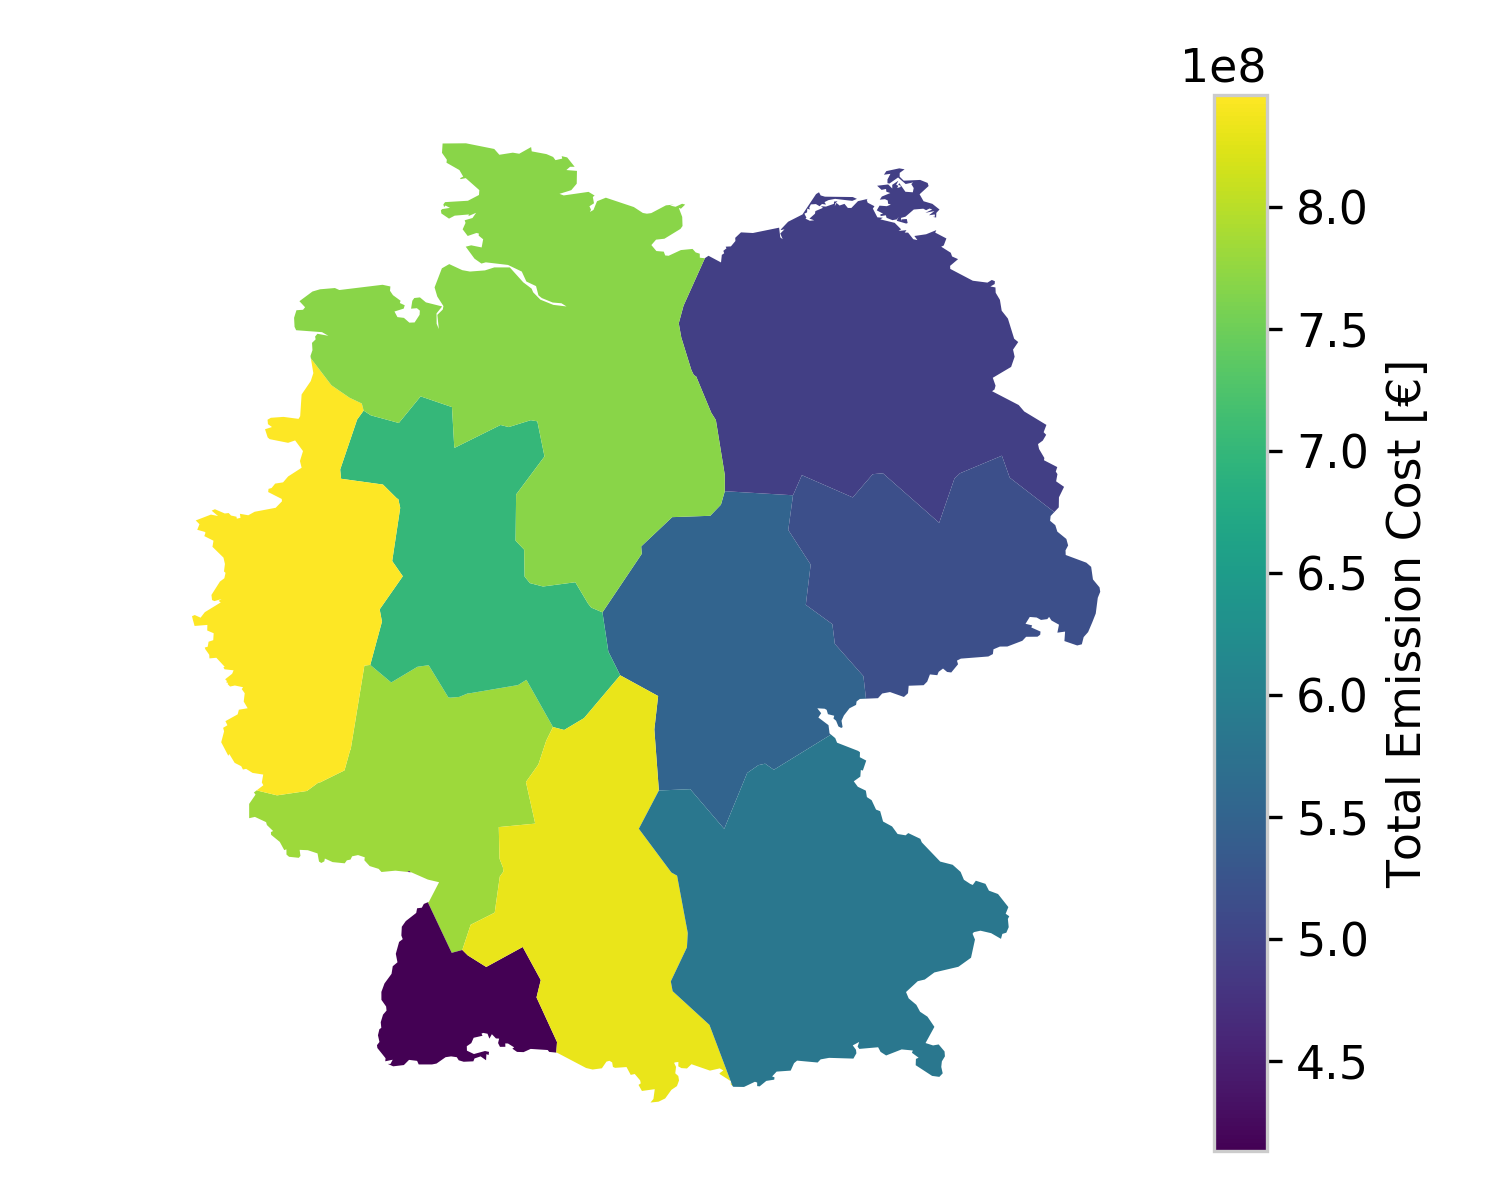
\includegraphics[width=\linewidth]{de50bf/maps_price_ptpf_net/co2_cost_total}
    \caption{Average electricity price for \textbf{allocated emission cost}, $\sum_t \allocateemissioncost$.}
    \label{fig:emission_cost}
\end{figure}

\begin{figure}
    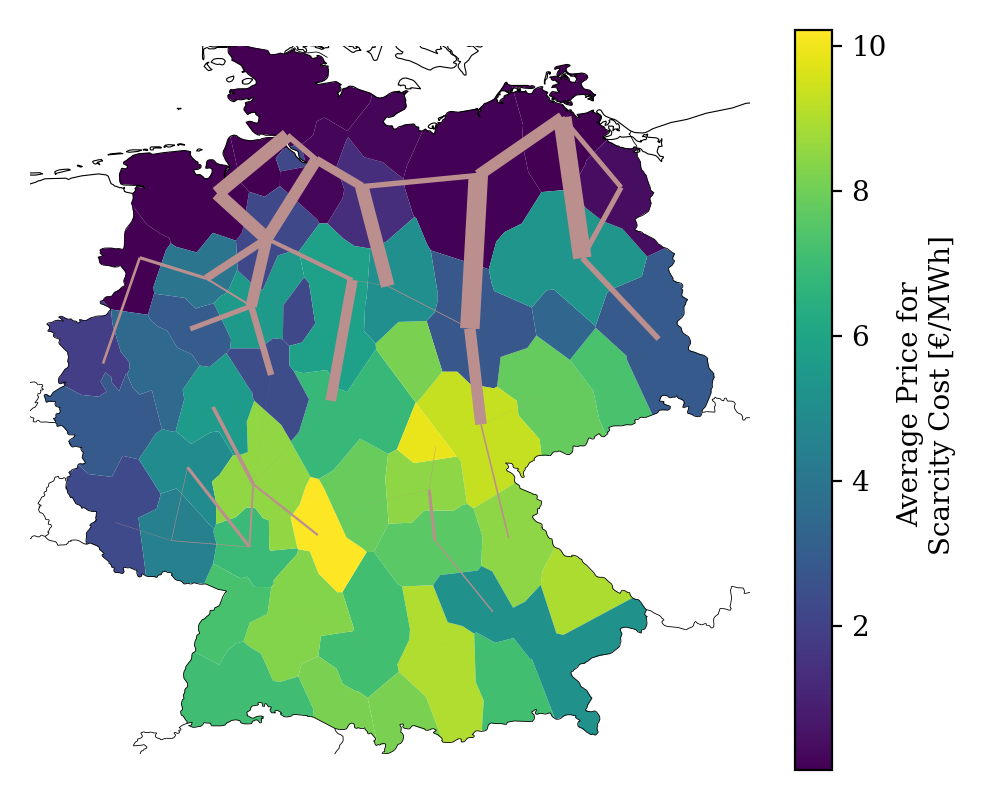
\includegraphics[width=\linewidth]{de50bf/maps_scarcity_price_ptpf_net/branch_scarcity_cost_total}
    \caption{Average electricity price for the \textbf{allocated scarcity cost}, $\sum_t \allocatescarcitycost$ for the transmission system, due to the upper transmission expansion limit of 25\%.}
    \label{fig:branch_scarcity_cost}
\end{figure}

\begin{figure*}
    \centering
    \begin{subfigure}[c]{.49\linewidth}
        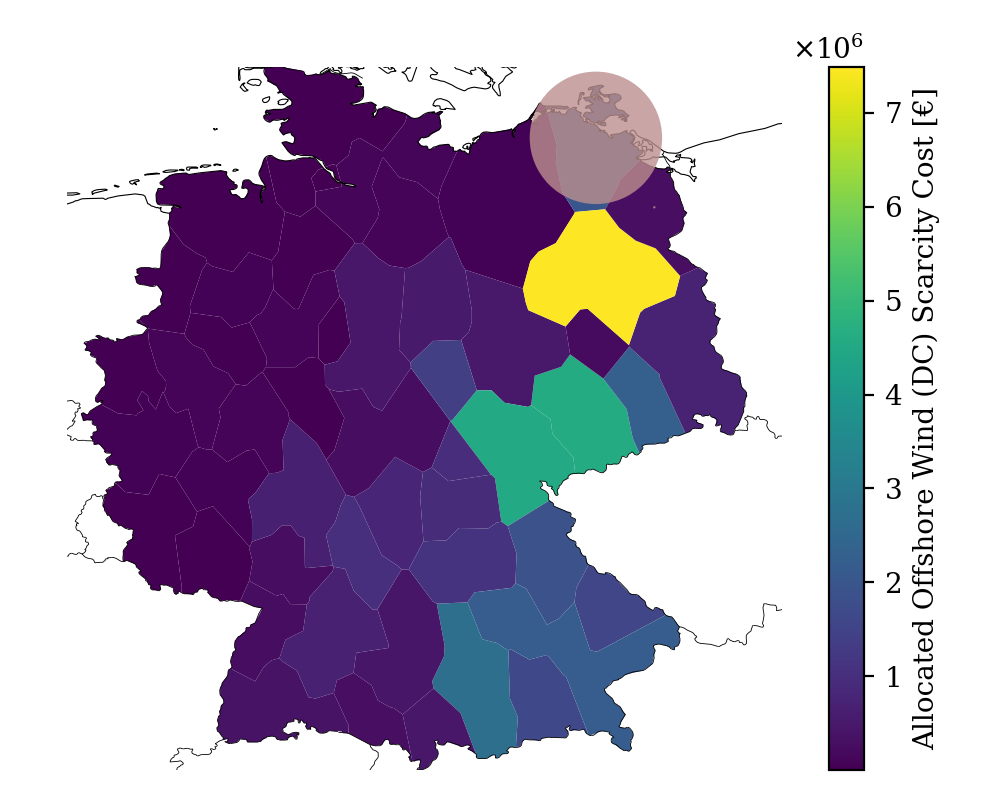
\includegraphics[width=\linewidth]{de50bf/maps_scarcity_price_ptpf_net/by_carrier/offwind-dc_generator_scarcity_cost}
        \subcaption{Offshore Wind}
        \label{fig:offwind-dc_generator_scarcity_cost}
    \end{subfigure}
    \begin{subfigure}[c]{.49\linewidth}
        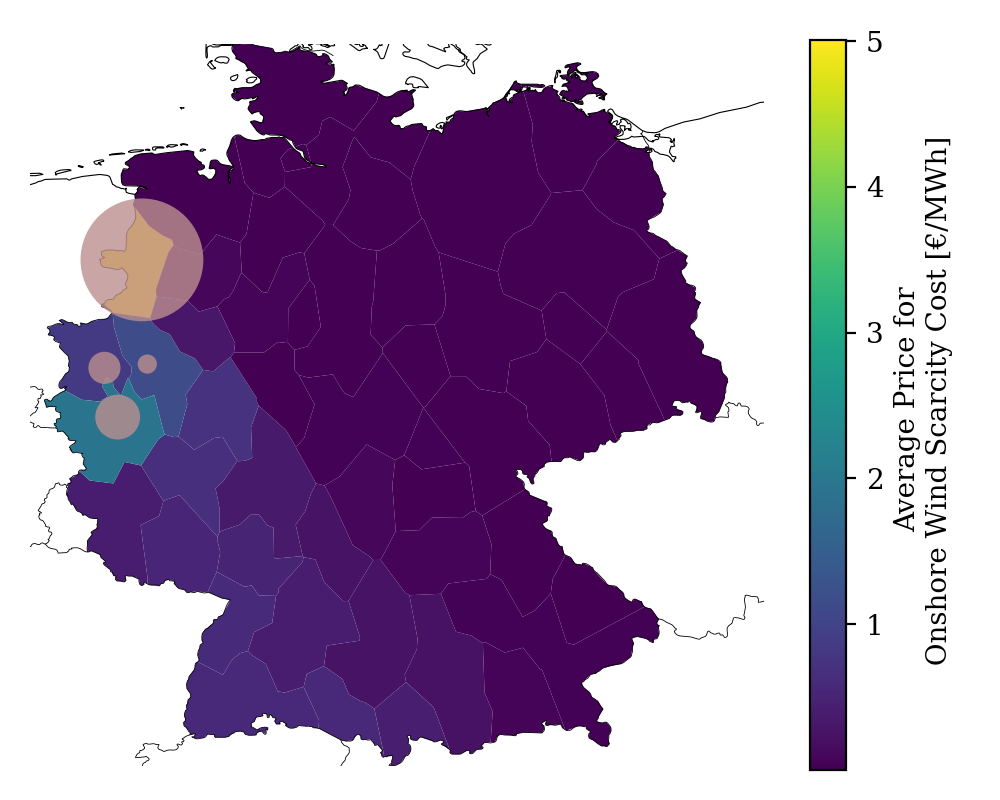
\includegraphics[width=\linewidth]{de50bf/maps_scarcity_price_ptpf_net/by_carrier/onwind_generator_scarcity_cost}
        \subcaption{Onshore Wind}
        \label{fig:onwind_generator_scarcity_cost}
    \end{subfigure}
    \begin{subfigure}[c]{.49\linewidth}
        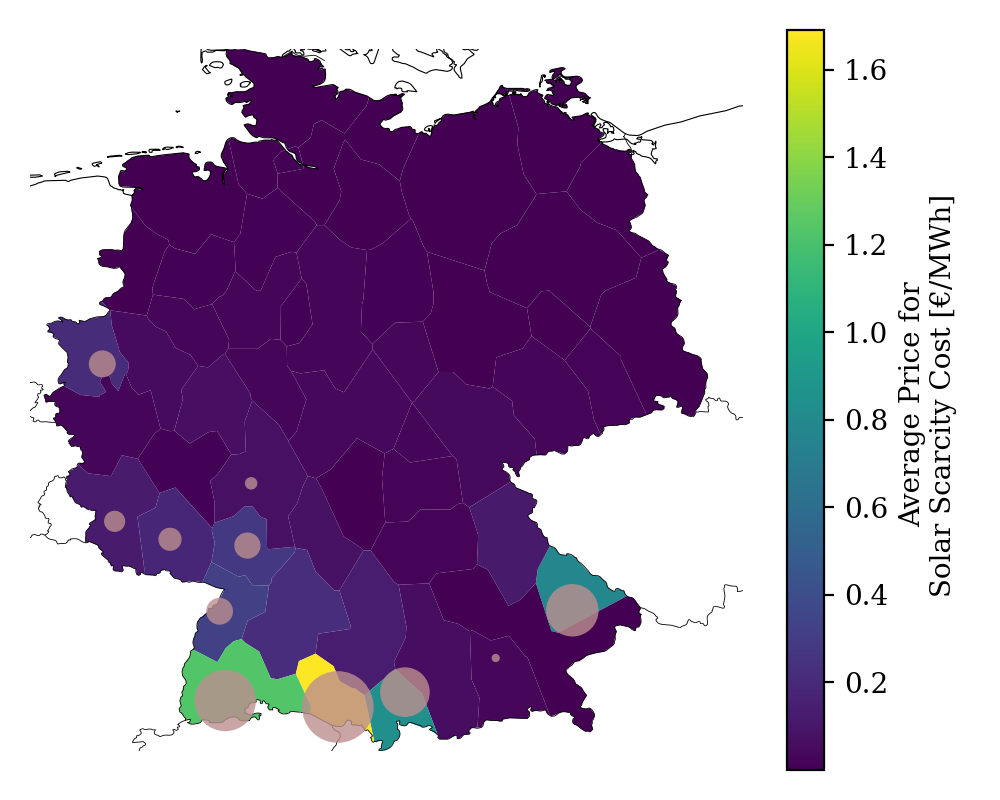
\includegraphics[width=\linewidth]{de50bf/maps_scarcity_price_ptpf_net/by_carrier/solar_generator_scarcity_cost}
        \subcaption{Solar}
        \label{fig:solar_generator_scarcity_cost}
    \end{subfigure}
    \begin{subfigure}[c]{.49\linewidth}
        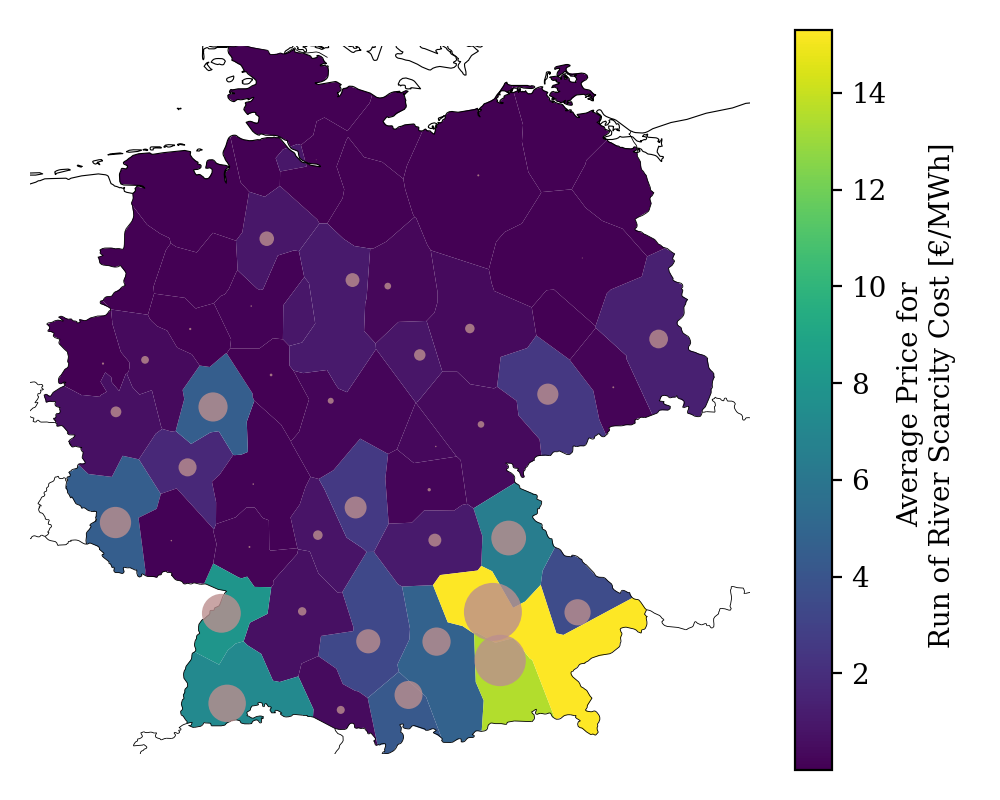
\includegraphics[width=\linewidth]{de50bf/maps_scarcity_price_ptpf_net/by_carrier/ror_generator_scarcity_cost}
        \subcaption{Run-of-River}
        \label{fig:ror_generator_scarcity_cost}
    \end{subfigure}
    \caption{Average electricity price for \textbf{allocated scarcity cost}, $\sum_t \allocatescarcitycost$, due to technology resource limits, for offshore wind, onshore wind,  solar, run-of-river. Average Allocated Scarcity Cost per MWh within the regions are indicated by the color, the revenue per production asset is given by the size of the circles at the corresponding bus.}
    \label{fig:scarcity_price}
\end{figure*}





\clearpage
\printbibliography




\end{document}
